\chapter{Event Reconstruction}

\section{Data Sample}

During 2011 the LHC delivered over 5.6 $fb^{-1}$ of integrated luminosity to ATLAS at a centre of mass energy of 7 TeV. Approximately 5.25 $fb^{-1}$ of this was recorded and, after data quality considerations, resulted in 4.665 $fb^{-1}$ of analysable data at a peak instantaneous luminosity of $3.65 * 10^{33}~cm^{-2}s^{-1}$. The 7 TeV run period was divided into sections corresponding to stable conditions, fixed instantaneous luminosity and bunch configuration; called periods. There were 13 periods in the 2011 data, labelled period A - period M. Some periods did not have stable detector conditions and as such are not considered in physics analyses, for example period A.

\begin{figure}[htbp!]
\begin{center}
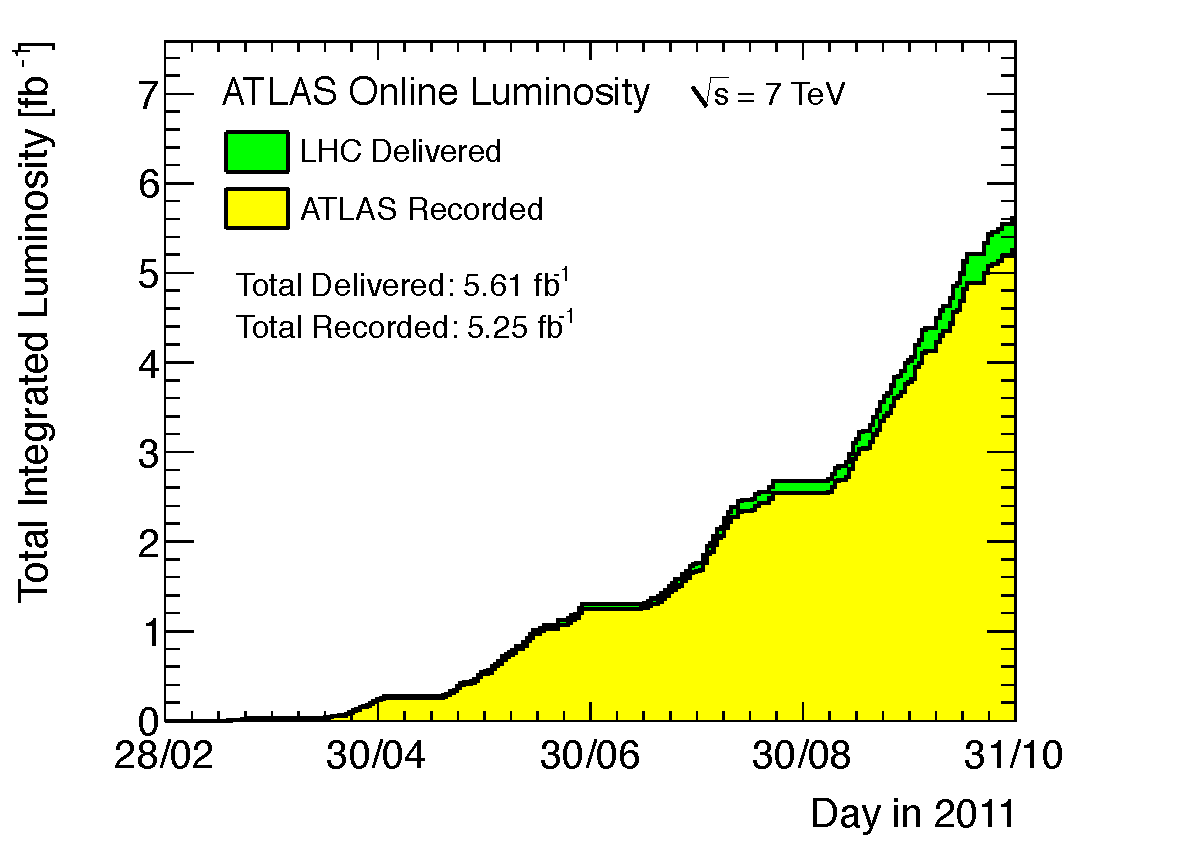
\includegraphics[width=75mm]{f/sumLumiByDay}
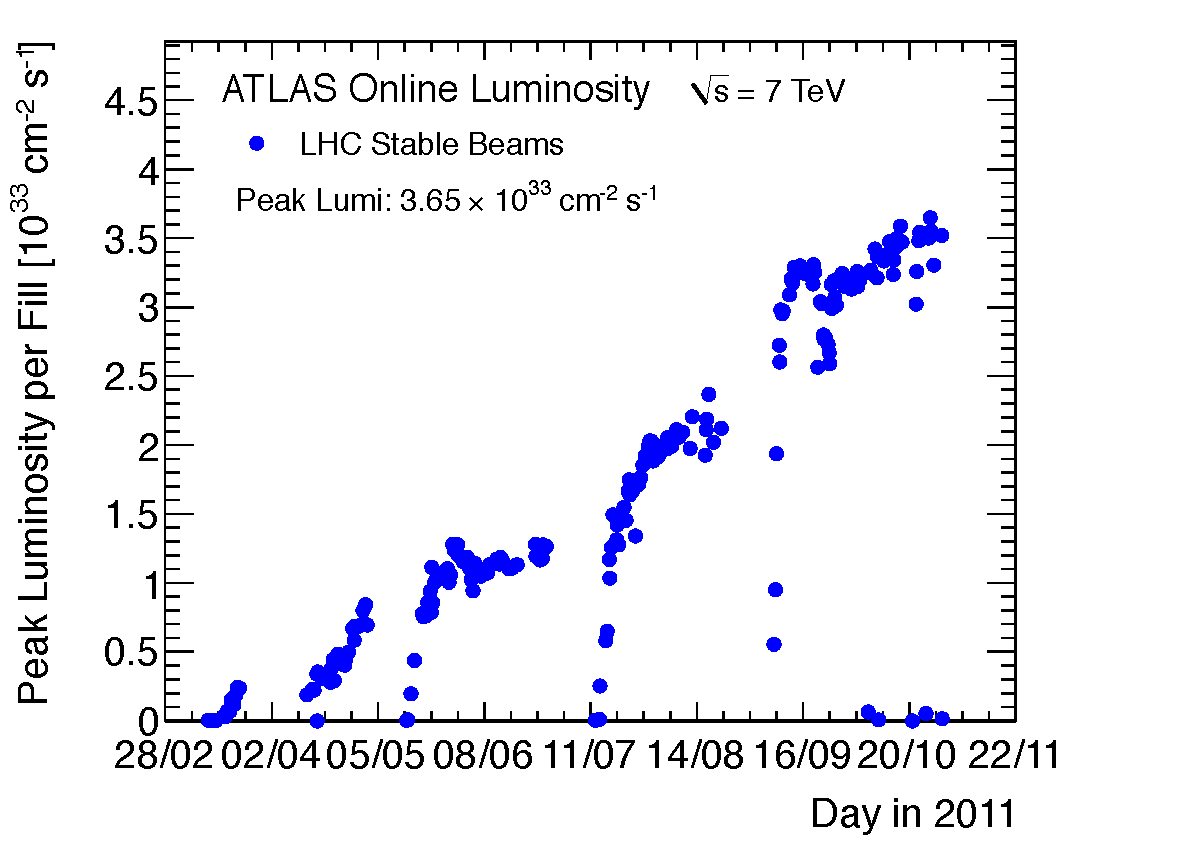
\includegraphics[width=75mm]{f/peakLumiByFill}
\end{center}
\caption{ATLAS integrated luminosity during 2011 \textit{(left)}. Peak instantaneous luminosity during the LHC7 run recorded by ATLAS \textit{(right)}.}
\label{fig:lumi}
\end{figure}

\section{Analysis Triggers}
\label{sec:analysis_trigger}

To select interesting \ttbar\ like events with high efficiency we use triggers based on single electron or muon signatures. Lepton signatures are plentiful in 7 TeV proton-proton collisions and in order to reduce the trigger rate to a manageable level it is necessary to impose a minimum \pt\ threshold on the trigger lepton. Electron triggers were required to have a trigger electron with minimum \pt\ of 20 GeV in periods B-J, a minimum \pt\ of 22 GeV in period K and either 22 GeV or 45 GeV in periods L-M, depending on other cuts in the trigger. The higher threshold of 45 GeV is used to accept events that are rejected by the lower threshold trigger in periods L-M. For Muons a minimum \pt\ cut of 18 GeV is required in all Periods.

In addition to \pt\ requirements, other cuts can be made to reduce trigger rate. For electrons these are based on calorimeter cluster information and inner detector trigger track isolation. For muons these are based on Muon Spectrometer trigger track isolation and other track quality parameters. Triggers at ATLAS have the definition of either \emph{loose}, \emph{medium}, or \emph{tight} depending on the efficiency of the cuts. \emph{Loose} triggers have high efficiency but low background rejection (also called ``purity"), whereas \emph{tight} triggers have lower efficiency but higher purity.\emph{Medium} triggers attempt to balancing efficiency with purity and as such are the triggers used in this analysis. In addition other affixes in the trigger name indicate a unique or unusual cut that is not always applied. For example in table \ref{tab:analysis_triggers}, the letters \emph{vh} in the electron triggers indicate that this trigger applied $\eta$ dependent cuts on hadronic isolation at trigger L1 \cite{LeptonTrigger}.

\begin{table}
	\begin{center}
	\begin{tabular}{|c|c|c|c|}
	\hline
	Data period & Int. Luminosity & Electron Trigger & Muon Trigger \\
	\hline
	period B-D    & $0.176~$fb$^{-1}$  & EF\_e20\_medium     & EF\_mu18        \\
	period E-H    & $0.938~$fb$^{-1}$  & EF\_e20\_medium     & EF\_mu18        \\
	period I      & $0.333~$fb$^{-1}$  & EF\_e20\_medium     & EF\_mu18        \\	
    period J      & $0.223~$fb$^{-1}$  & EF\_e20\_medium     & EF\_mu18\_medium\\
	period K      & $0.583~$fb$^{-1}$  & EF\_e22\_medium     & EF\_mu18\_medium\\
	period L-M    & $2.402~$fb$^{-1}$  & EF\_e22vh\_medium1 OR EF\_e45\_medium1     & EF\_mu18\_medium\\
	\hline
	\end{tabular}
	\end{center}
	\caption{Table of analysis triggers used for data taking in the 7 TeV data. Note that \emph{medium1} and \emph{medium} are two distinct triggers.}
	\label{tab:analysis_triggers}
\end{table}


\section{Event Selection}
\label{sec:event_selection}

Kinematic cuts and data quality requirements are imposed on the data and MC samples in order to optimise the signal to background ratio (i.e. to bias the sample towards the signal events and reject background events). A list of the cuts employed, along with the motivation for these cuts follows. 

\subsection*{Selection}
\begin{itemize}

  \item \textbf{Passed single lepton trigger}: Events are required to have fired either an electron or muon trigger, as described in section \ref{sec:analysis_trigger}.

  \item \textbf{Exactly two opposite sign leptons}: Exactly two well reconstructed leptons are required; either two electrons, muons or one electron and one muon. All lepton pairs are must have opposite sign charge.

  \item \textbf{Two or more selected jets}: We require at least two well reconstructed jets in each event, though these need not be tagged as having b flavour. When combined with the lepton multiplicity requirement, this cut removes most other SM physics signals from the selection, particularly in the \emu channel where there are no significant Drell-Yan contributions. Many background signals require extra radiated jets either from pileup or NLO radiative corrections in order to imitate the signal kinematics and therefore this cut is highly efficient at accepting signal events whilst reducing background signals, as can be seen in figures \ref{fig:dilep_control_sig_ee}, \ref{fig:dilep_control_sig_mumu} and \ref{fig:dilep_control_sig_emu}.

  \item \textbf{\etmiss $>$ 60 \GeV}: (\ee\ and \mumu\ channels only) This kinematic cut reduces contribution from Drell-Yan events (where there are no neutrinos is the hard scatter to create missing energy) and some diboson events by requiring a large amount of missing transverse energy. For \ttbar\ dilepton events the efficiency of this cut is very high due to the two neutrinos in the dilepton final state, illustrated in figures \ref{fig:dilep_control_sig_ee}, \ref{fig:dilep_control_sig_mumu}. This cut is not motivated in the \emu\ channel illustrated in \ref{fig:dilep_control_sig_emu}.

  \item \textbf{Invariant mass $>$ 15 \GeV}: (\ee\ and \mumu\ channels only)  Invariant mass is defined as the invariant mass between the two selected leptons in the event. Low energy Drell-Yan events and meson production such as $J/\Psi$ can enter the selection by decaying to two opposite sign leptons but typically have a low invariant mass and are rejected by this cut. The invariant mass of the \ttbar\ system tends to peak at much higher values and so this does not have a damaging effect on signal acceptance. This is shown in figures \ref{fig:dilep_control_sig_ee} and \ref{fig:dilep_control_sig_mumu}. 

  \item \textbf{$H_T >$ 130 \GeV }: (\emu\ channel only) $H_T$ is defined as the scalar sum of the transverse energy of all selected leptons and jets in the event. This cut is only applied in the \emu\ channel and can loosely be describe as requiring a large amount of energetic activity in the event. This cut rejects events with lower energy (for example a diboson event whose extra radiated jets are low in energy but still pass the jet $p_T$ cut.

  \item \textbf{Z Boson Veto }: (\ee and \mumu channels only) Events with an invariant mass that is less than 10 GeV away from the Z Boson pole mass of 91 GeV are rejected. This cut reduces a large amount of the Drell-Yan $\rightarrow \ee$ or \mumu\ background. Events in which Z Bosons decay to two tau leptons (that then decay leptonically) have a broad invariant mass spectrum that peaks at lower values, as shown in figures \ref{fig:dilep_control_sig_ee} and \ref{fig:dilep_control_sig_ee}, and a similar cut to suppress this background would result in an unacceptable loss of signal statistics. This cut also has difference acceptance in the standard model spin sample and the uncorrelated spin sample. This reason for this is that in the uncorrelated sample, the leptons typically have a larger separation in $\phi$ and hence a higher invariant mass. This results in the efficiency of this cut being higher for the uncorrelated sample than it is for the standard model sample, but this effect is considered in the extraction procedure later and is typically quite small (on the order of 3\%).

In the dominant channel for dilepton events (the \emu\ channel), there are no cuts on invariant mass as there are no standard model processes where Z Bosons may violate lepton flavour conservation and decay to an electron and a muon.

  \item \textbf{Cosmic Rejection}: Events are rejected if two muon tracks are back to back in phi (i.e. $\Delta\phi > 3.1$) and if the point of closest approach to the vertex is greater than 5mm, with both tracks on the same side of the detector. 

  \item \textbf{Data Quality Cuts}: An event in data is required to have been included in a good run list (GRL). These GRLs are generated centrally by ATLAS and reject events where data quality was deemed to be poor. Physics subgroups may impose their own requirements if appropriate. In the case of a predominantly jet based analysis, bad data quality the inner detector may be a tolerable defect, whereas for a muon based Drell-Yan selection the calorimeter information may not be necessary. For top analyses we require that the entire detector is online and that the data quality has been assessed to be good by the relevant experts (see section \ref{sec:dq}).

A reconstructed vertex, with at least three tracks, is required to have been identified as a primary vertex and not originating from pileup. 

In 2011 a tower of the ATLAS Liquid Argon calorimeter was disabled creating a hole in the acceptance. In the portions of effected data, events are rejected where it is believed that a jet has been mismeasured due to this fault. In addition the effect of this is taken into account in the detector simulation and reconstruction of \etmiss .

  \item \textbf{Passed Truth Cuts}: In signal MC events, we require that the selected event be a true dilepton \ttbar\ event, and that the two reconstructed leptons correspond to the true leptons for this event and are not from a secondary process (such as a semi-leptonic b decay). This avoids double counting contributions from fake or mismeasured leptons, which are estimated separately using a data driven method. 

\end{itemize}

With the application of all cuts the contribution of background to the selection is approximately 20\%. With the addition of a single b-jet requirement (b-tag) this can be reduced to 10\%, with only single top events being an effective background. The cost in statistics for utilizing b-tagging  to signal events is quite large (on the order of $~20$\%). Though the 7 TeV has ample statistics in dileptonic \ttbar\ events, the cut effectively removes the \ee\ channel as a useful dataset and so it is not included in the final selection. For future results with higher statistics and higher centre of mass energies it may prove useful to impose a double b-tag, which effectively removes most SM background events. 

\todo[inline]{Yields and explanation of efficiencies in \ee, \mumu and \emu}

\subsection{Signal Monte Carlo}
Signal \ttbar\ events are generated using the MC@NLO generator interfaced with HERWIG and JIMMY for parton showering (PS) and underlying event (UE) simulation respectively. MC@NLO generates both top quarks, the W and b particles, and the subsequent W decay. HERWIG then showers the b quarks and W boson daughters (in the dilepton case electrons, muons or taus). By adjusting the point at which HERWIG initiates the showering and decay we can effectively remove spin correlation from out MC. If HERWIG is allowed to decay the top quarks then they will be treated as unpolarised and uncorrelated. In this manner we generate 15 million \ttbar\ events with spin correlation (semi-leptonic and dileptonic) and 10 million events without spin correlation (again without fully hadronic decays). This technique has the side effect of the top quarks in the uncorrelated case being treated on shell and hence not including an intrinsic width. The effect of this is describe further in section \ref{sec:systematics} and is estimated to be negligible.

Signal events are also generated with POWHEG interfaced to HERWIG or PYTHIA, as well as ALPGEN interfaced to HERWIG, all using JIMMY for UE modelling. These samples are only used for the estimation of systematic uncertainties.

Care must be taken when interfacing HERWIG with different ME generators. In certain combinations HERWIG will not pass tau polarisation information correctly\footnote{Tau decays in HERWIG are handled by the TAUOLA program.} and tau decays will be treated as unpolarised, effectively making an event with a tau decay appear uncorrelated. This was noted in all ATLAS MC samples and is only present in the POWHEG + HERWIG implementation. In a similar analysis performed by CMS, this was not accounted for in the signal MC and became a dominant source for systematic uncertainty.  

Fully hadronic \ttbar\ decays are not considered in our samples as these events can only contribute to the selection via non prompt leptons and hence fall under the definition of ``fake" lepton. 

\subsection{Data driven background estimation}

Ideally one would prefer to estimate as many background processes as possible using data driven techniques as these suffer less from theoretical uncertainties than MC alone, which can be large in some cases. In this selection, the normalisation of Drell-Yan Monte Carlo is derived by comparing the normalisation with data in a Drell-Yan dominated control region (see section \ref {sec:drell_yan}). Experimentally mismeasured leptons, or 'fake leptons' as they are more commonly known, are also estimated using a data driven technique. These are defined as leptons arising from photon conversions, mismeasured jets (as electrons) and leptons arising from heavy flavour decays inside jets. Leptons arising from hard scatter leptonic tau decay are not considered as fakes. 

\subsubsection*{Matrix Method for determining fake lepton background}

The matrix method is used to determine the shape and normalisation of backgrounds due to fake leptons \cite{fakes}\cite{topwg}. It defines two lepton definitions, \emph{loose} and \emph{tight}. The \emph{tight} selection is the selection used for analysis (see section \ref{sec:electrons},\ref{sec:muons}). The \emph{loose} selection is the same as the \emph{tight} selection but with isolation requirements relaxed (in the case of electrons) or removed (in the case of muons). 
\todo[inline]{Describe the motivation for matrix method better}
We also define two efficiencies, one for fake leptons and one for real leptons (i.e. prompt hard scatter) such that:

\begin{equation}
	\textcolor{Blue}{\mathbf{r_i}} = \epsilon_{real} = \frac{  N^{\text{tight}}_{\text{real}} }{ N^{\text{loose}}_{\text{real}} }~~~~\&~~~~\textcolor{Red}{\mathbf{f_i}} = \epsilon_{\text{fake}} = \frac{ N^{\text{tight}}_{\text{fake}} }{ N^{\text{loose}}_{\text{fake}}}
	\label{eq:fake_eff}	
\end{equation}

The $\epsilon_{real}$ is measured using a tag and probe technique in Z boson events, $\epsilon_{fake}$ is measured from control regions with high contributions from fake leptons, for example a same sign low \etmiss\ selection. 

The number of events with different lepton quality definitions may then be expressed as a matrix:

\begin{equation}
\begin{bmatrix}
%N^{\textcolor{blue}{\mathbf{tt}}} \\
%N^{\textcolor{blue}{\mathbf{t}}\textcolor{red}{\mathbf{l}}} \\
%N^{\textcolor{Red}{\mathbf{l}}\textcolor{blue}{\mathbf{t}}} \\
%N^{\textcolor{Red}{\mathbf{ll}}} \\
N^{\mathbf{tt}} \\
N^{\mathbf{t}\mathbf{l}} \\
N^{\mathbf{l}\mathbf{t}} \\
N^{\mathbf{ll}} \\
\end{bmatrix} 
= \mathbf{M}
\begin{bmatrix}
%N^{\textcolor{Red}{\mathbf{ll}}}_{\textcolor{Green}{\mathbf{rr}}} \\
%N^{\textcolor{Red}{\mathbf{ll}}}_{\textcolor{Green}{\mathbf{r}}f} \\
%N^{\textcolor{Red}{\mathbf{ll}}}_{fr} \\
%N^{\textcolor{Red}{\mathbf{ll}}}_{ff} \\

%N^{\mathbf{ll}}_{\textcolor{Blue}{\mathbf{rr}}} \\
%N^{\mathbf{ll}}_{\textcolor{Blue}{\mathbf{r}}\textcolor{Red}{\mathbf{f}}} \\
%N^{\mathbf{ll}}_{\textcolor{Red}{\mathbf{f}}\textcolor{Blue}{\mathbf{r}}} \\
%N^{\mathbf{ll}}_{\textcolor{Red}{\mathbf{ff}}}\\

N^{\mathbf{ll}}_{\rone\rtwo}\\
N^{\mathbf{ll}}_{\rone\ftwo}\\
N^{\mathbf{ll}}_{\fone\rtwo}\\
N^{\mathbf{ll}}_{\fone\ftwo}\\
\end{bmatrix}
\label{eq:fake}
\end{equation}

\begin{equation}
\mathbf{M} = 
\begin{bmatrix}
%r_1 r_2         & r_1f_2         & f_1r_2         & f_1f_2 \\
%r_1(1-r_2)     & r_1(1-f_2)     & f_1(1-r_2)     & f_1(1-f_2) \\
%(1-r_1)r_2     & (1-r_1)f_2     & (1-f_1)r_2     & (1-f_1)f_2 \\
%(1-r_1)(1-r_2) & (1-r_1)(1-f_2) & (1-f_1)(1-r_2) & (1-f_1)(1-f_2) \\

\rone \rtwo          & \rone \ftwo         & \fone \rtwo         & \fone \ftwo \\
\rone (1-\rtwo )     & \rone (1-\ftwo )    & \fone (1- \rtwo )   & \fone (1- \ftwo ) \\
(1-\rone )\rtwo      & (1-\rone )\ftwo     & (1-\fone )\rtwo     & (1-\fone )\ftwo  \\
(1-\rone )(1-\rtwo ) & (1-\rone )(1-\ftwo )& (1-\fone )(1-\rtwo )& (1-\fone )(1-\ftwo )\\

%(1-r_1)(1-r_2) & (1-r_1)(1-f_2) & (1-f_1)(1-r_2) & (1-f_1)(1-f_2) \\
\end{bmatrix}
\end{equation}

Where $N$ is the number of events passing the selection, the upstairs notation indicates the tightness of the selection (t = \emph{tight}, l= \emph{loose}) for each lepton, and the downstairs notation is if the lepton was real or fake. For the estimate of the fake contribution to the signal region we are interested in determining the number of events with at least one fake lepton contaminating the $N^{tt}$ selection using observable properties such as the real and fake efficiencies for leptons, and the number of events with leptons passing \emph{tight} or \emph{loose} selections and with now knowledge on if these leptons were fake or real. We may extract this by inverting the matrix M such that and rearranging equation \ref{eq:fake} such that:

\begin{align}
N^{tt}_{fake} =&~ N^{tt}_{rf} + N^{tt}_{fr} + N^{tt}_{ff} \\
              =&~ \rone \ftwo N^{ll}_{rf} + \fone \rtwo N^{ll}_{fr} + \fone \ftwo N^{ll}_{ff} \\
              =&~ \alpha \rone \ftwo [(\fone -1)(1-\rtwo )N^{tt} + (1-\fone )\rtwo N^{tl} + \fone (1-\rtwo )N^{lt} - \fone \rtwo N^{ll}] \nonumber \\
               +&~ \alpha \fone \rtwo [(\rone -1)(1-\ftwo )N^{tt} + (1-\rone )\ftwo N^{tl} + \rone (1-\ftwo )N^{lt} - \rone \ftwo N^{ll}] \nonumber \\
               +&~ \alpha \fone \ftwo [(1-\rone )(1-\rtwo )N^{tt} + (\rone - 1)\rtwo N^{tl} + \rone (\rtwo  -1)N^{lt} + \rone \rtwo N^{ll}]
%              =&~ r_1f_2N^{ll}_{rf} + f_1r_2N^{ll}_{fr} + f_1f_2N^{ll}_{ff} \\
%              =&~ \alpha r_1f_2[(f_1-1)(1-r_2)N^{tt} + (1-f_1)r_2N^{tl} + f_1(1-r_2)N^{lt} - f_1r_2N^{ll}] \nonumber \\
%               +&~ \alpha f_1r_2[(r_1-1)(1-f_2)N^{tt} + (1-r_1)f_2N^{tl} + r_1(1-f_2)N^{lt} - r_1f_2N^{ll}] \nonumber \\
%               +&~ \alpha f_1f_2[(1-r_1)(1-r_2)N^{tt} + (r_1 - 1)r_2N^{tl} + r_1(r_2 -1)N^{lt} + r_1r_2N^{ll}]
\end{align}

where

\begin{equation*}
\alpha = \frac{1}{(\rone - \fone )(\rtwo -\ftwo )}
%\alpha = \frac{1}{(r_1 - f_1)(r_2-f_2)}
\end{equation*}

We can now extract $N^{tt}$, $N^{tl}$, and $N^{ll}$ from the data in our signal selection and use our derived real and fake efficiencies to estimate the contributions from fake leptons. In practice this can be applied not as just single numbers but as distributions (such as our observable distributions) and the efficiencies parametrised as functions of $\eta$, $p_T$ or $\Delta R$ with closest jet. This method requires that $\epsilon_{fake}$ and $\epsilon_{real}$ are different, or at least the definitions of of tight and loose are different, and therefore care must be taken to maintain this assumption whilst maintaining a reasonable lepton definition.

\subsubsection*{Normalisation of Drell-Yan MC using data}
\label{sec:drell_yan}

In the \ee\ and \mumu\ channels the shape of background contributions from \Zee\ or \Zmm\ events is taken from Monte Carlo. The normalisation is taken by comparing data events to MC events in a region dominated by \Zll\ events (see section \ref{sec:drell_yan}) using equation \ref{eq:drell_yan}. In this control region (CR) non Drell-Yan background (including \Ztautau\ ) are subtracted from the data to approximate the number of \Zee\ or \Zmm\ events seen in data.

 \begin{equation}
   \label{eq:drell_yan}
   N_{Z/\gamma^* + jets} = \frac{Data^{(CR)} - MC_{other}^{(CR)}}{MC_{Z/\gamma^* + jets}^{(CR)}} \times MC_{Z/\gamma^* + jets}^{(SR)}
 \end{equation} 

 \begin{table}[htb]
   \begin{center}
     \begin{tabular}{|c|c|c|}
       \hline
       Process & \ee & \mumu \\
       \hline
       Data (CR)         &  3157.0  & 9194.0   \\
       MC$_{DY}$ (CR)    &  2723.07 & 7586.28  \\
       MC$_{Other}$ (CR) &   409.40 &  711.40  \\
       \hline
       Scale Factor      &   1.009  &  1.118   \\
       MC$_{DY}$ (SR)    &   20.67  &   74.70   \\
       Scaled MC         &   20.86  &   83.52  \\
       \hline
     \end{tabular}
   \end{center}
   \caption{Yields for the estimates of the $Z/\gamma^*$+jets background
     with the data-driven and Monte Carlo methods using non-isolated electron fakes. Yields are shown in the Z dominated control region (CR) and in the signal region (SR).} %and total uncertainties
   \label{tab:dilep_znorm}
 \end{table}

\subsection{Monte Carlo background contributions}

\begin{figure}[htbp!]
\begin{center}
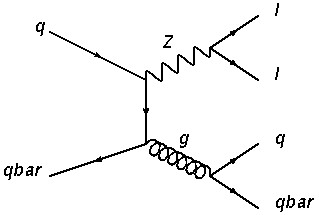
\includegraphics[width=75mm]{f/Z_jets}
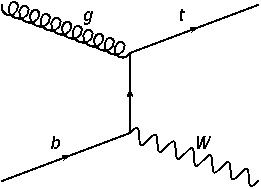
\includegraphics[width=65mm]{f/single_top_Wt}
\end{center}
\caption{Feynman diagrams of some of the dominant background SM processes to dileptonic \ttbar\ events; Z + jets \emph{(left)} and single top quark production \emph{(right)}}
\label{fig:background_feynman}
\end{figure}

\todo[inline]{Update Yield Numbers}
\todo[inline]{Make nicer Feynman Diagrams}

Backgrounds that cannot be derived directly or indirectly from the data are determined from Monte Carlo samples. Events coming from single top production are modelled using MC@NLO interfaced with HERWIG and JIMMY. Only the associated production channel (Wt channel) is considered as only this can imitate the signal events without the addition of a fake lepton. 

Drell-Yan events are generated using the leading order generator ALPGEN interfaced to HERWIG and JIMMY for PS and UE respectively. Events are simulated with 0 - 5 (incl.) additional partons in both the high invariant mass regime (40 and 2000 GeV) and the low invariant mass regime (between 10 $\rightarrow$ 40 GeV).For dielectron and dimoun events the normalisation is derived from data (see section \ref{sec:drell_yan}). For ditau events, the normalisation is taken from the cross section used in the MC generator.

Events from dibosonic processes (WW, WZ, ZZ) are also modelled using ALPGEN + HERWIG/JIMMY. In these cases events are generated with 0, 1, 2 or 3 (inc.) additional partons. Each MC sample derived from pure MC has an associated systematic uncertainty on the cross section. This is described further in section \ref{sec:systematics}.

\section{Selection on 7 TeV data}

Figures \ref{fig:ee_control_dy} to \ref{fig:dilep_lep2_emu} show comparisons between simulated events and observed events in the signal region and background dominated control regions. Good agreement is observed in all distributions. The uncertainty on the normalisation of the simulated samples is also shown. The procedure for estimating this uncertainty is described in section \ref{sec:systematics}. A small deviation in the jet multiplicity distribution at four or more jets is observed in the signal region. The cause of this was found to be the MC@NLO generator used to simulate the signal \ttbar\ events. MC@NLO underestimated the number of jets in the signal events causing the observed discrepancy. The problem is largely one of normalisation and significant changes in the shapes of distributions due to this effect are not observed. The observed yields in data and MC are summarised in table \ref{tab:dilep_cutflow}.

\begin{table}[htbp!]
     \begin{center}
     \begin{tabular}{c c c c}
     \hline
      & \ee & \mumu & \emu \\
     \hline
     $Z+$jets (DD)                        &  20.9 &   83.5 &  -     \\
     $Z(\rightarrow \tau \tau)$+jets (MC) &  18.5 &   68.4 &  175.3 \\
     Fake leptons (DD)                    &  19.8 &   27.7 &   98.4 \\
     Single top (MC)                      &  31.2 &   84.0 &  228.5 \\
     Diboson (MC)                         &  22.9 &   61.4 &  177.6 \\
     \hline
     Total (non-\ttbar)                   & 113.3 &  325.0 &  679.8 \\
     \ttbar\ (MC)                         & 583.9 & 1673.4 & 4413.6 \\
     \hline
     Expected                             & 697.2 & 1998.4 & 5093.4 \\
     Observed                             & 740   & 2058   & 5329   \\
    
     \hline
     \end{tabular}
     \end{center}
     \caption{Observed events in Data and MC in the dilepton \ttbar\ selection. Backgrounds estimated from Monte Carlo are indicated with the (MC) suffix, whereas backgrounds estimated by data driven techniques are indicated with a (DD) suffix.}
     \label{tab:dilep_cutflow}
     \end{table}

\todo[inline]{Add normalisation uncertainties to all plots.}
\todo[inline]{Need to backup this statements about it not effecting the shape.}

\begin{figure}[hbtp!]
	 \begin{center}
         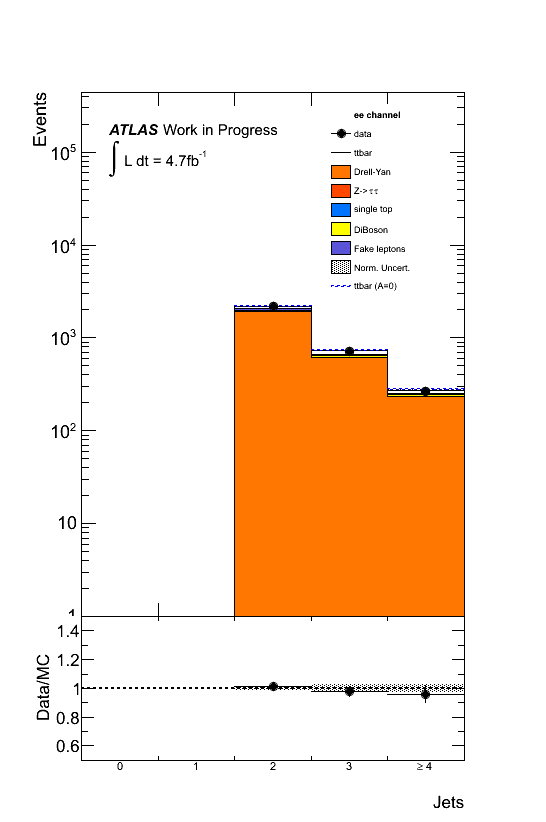
\includegraphics[width=50mm]{f/ee_dy_njet_central_double}
         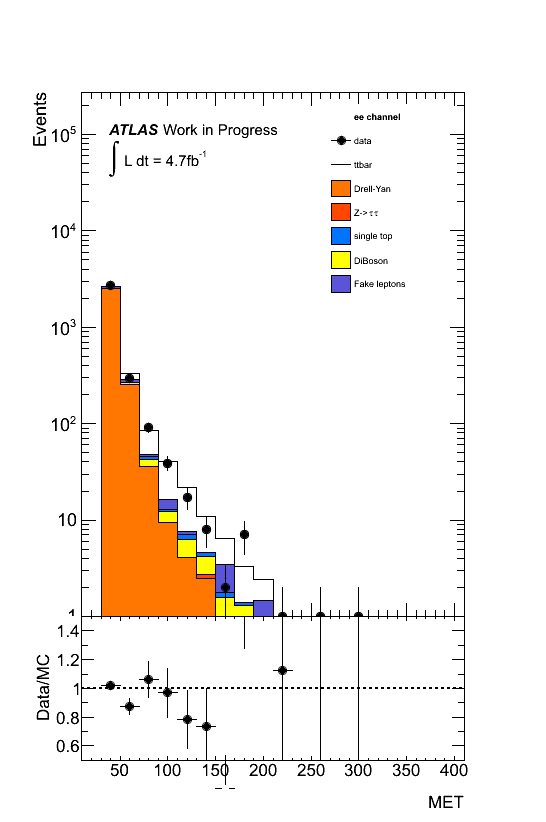
\includegraphics[width=50mm]{f/ee_dy_met_central_double}
         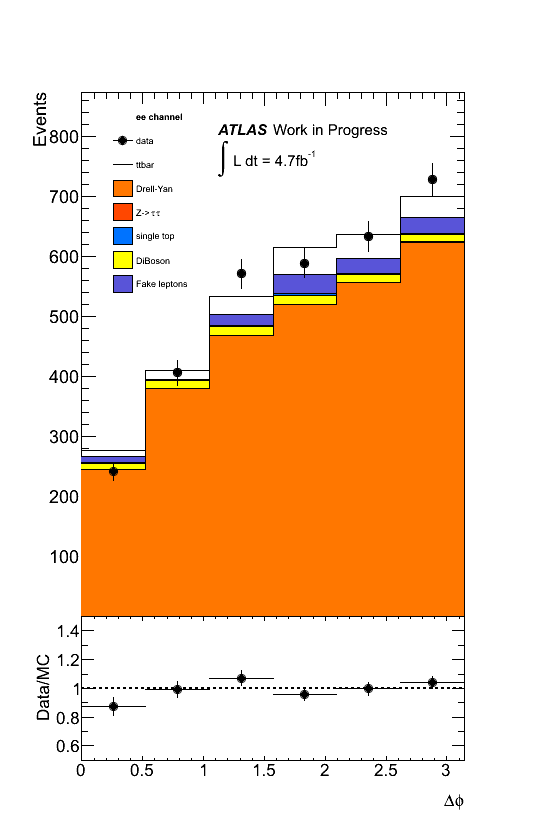
\includegraphics[width=50mm]{f/ee_dy_delta_phi_central_double}
       \end{center}
       \caption{Distributions for the \ee\ channel showing the jet multiplicity, reconstructed Z boson $p_{T}$, and $\Delta\phi$ analysis variable in the Drell-Yan control region.}
     \label{fig:ee_control_dy}
\end{figure}

\begin{figure}[hbtp!]
	 \begin{center}
         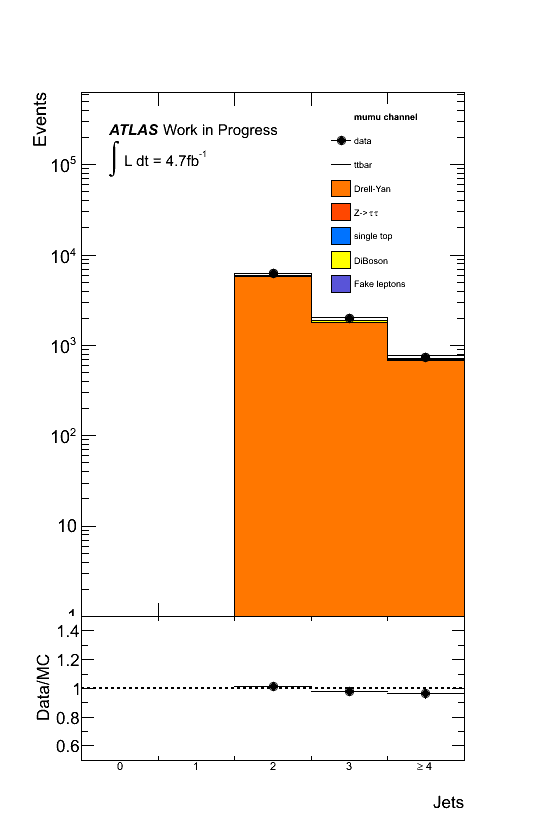
\includegraphics[width=50mm]{f/mumu_dy_njet_central_double}
         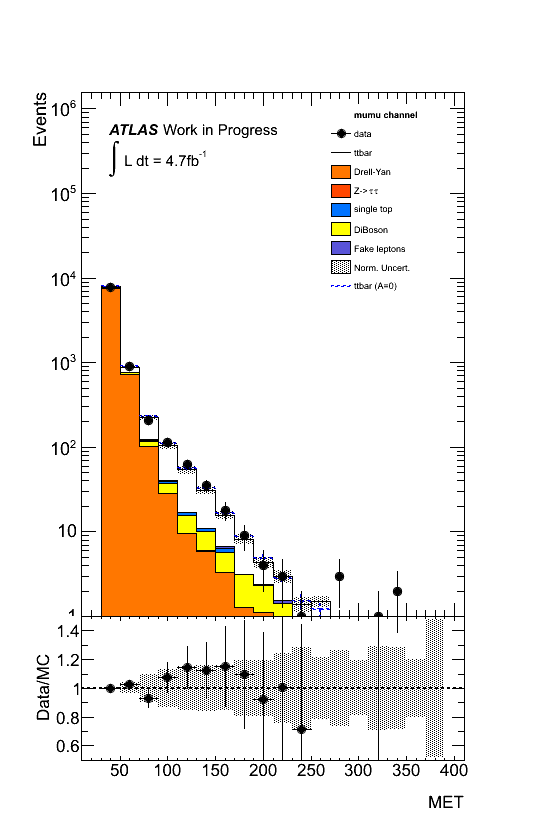
\includegraphics[width=50mm]{f/mumu_dy_met_central_double}
         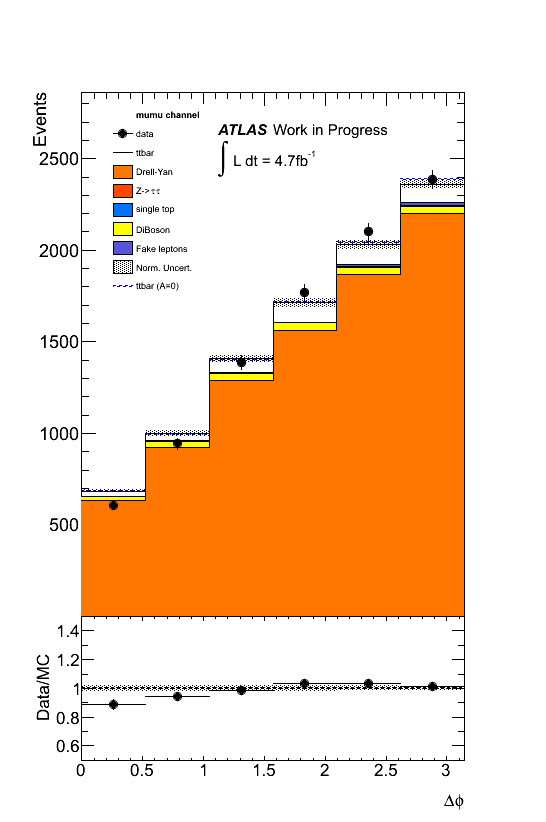
\includegraphics[width=50mm]{f/mumu_dy_delta_phi_central_double}
       \end{center}
       \caption{Distributions for the \mumu\ channel showing the jet multiplicity, reconstructed Z boson $p_{T}$, and $\Delta\phi$ analysis variable in the Drell-Yan control region.}
     \label{fig:mumu_control_dy}
\end{figure}
    
%     \begin{figure}[htbp!]
%     \begin{center}
%     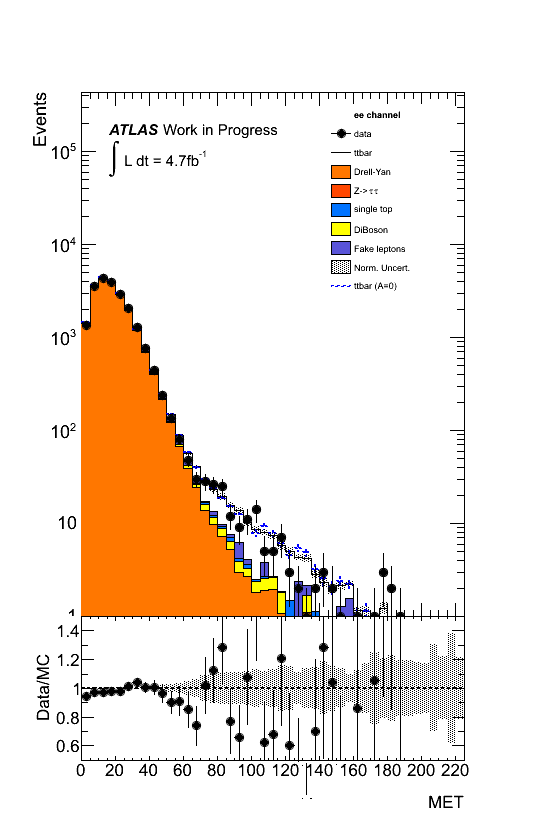
\includegraphics[width=50mm]{f/ee_control_met_central_double}
%     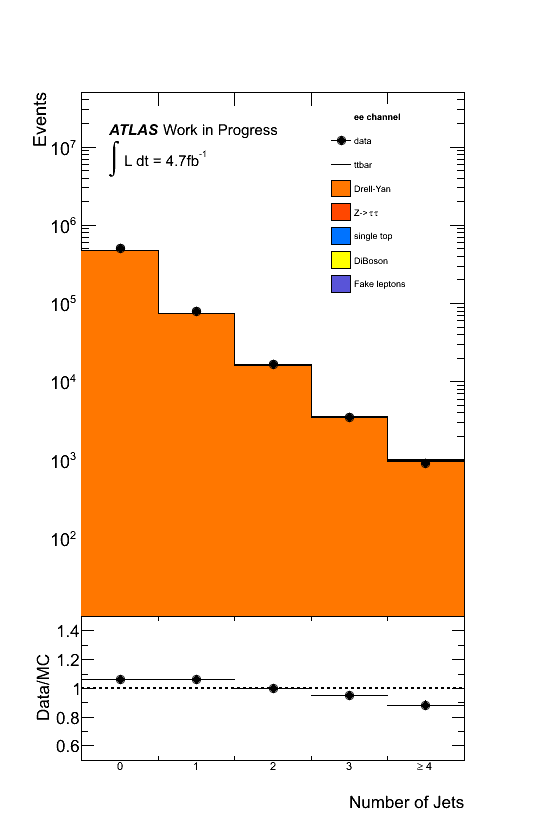
\includegraphics[width=50mm]{f/ee_control_njet_central_double}
%     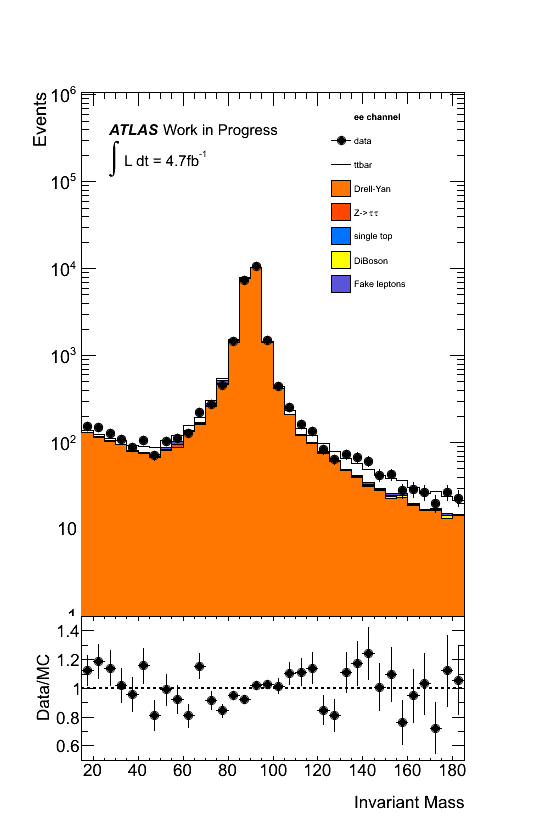
\includegraphics[width=50mm]{f/ee_control_invmass_central_double}
%     \end{center}
%     \caption{Control plots for the \ee\ channel.  \etmiss\ distribution in events with a dilepton mass inside the $Z$-boson mass window and at least two jets (left).  The number of jets in events with a dilepton mass inside the $Z$-boson mass window and \etmiss\ $< 40$~GeV (centre) and the invariant mass of opposite-sign lepton pairs in events with at least two jets and with \etmiss\ $< 40$~GeV (right).}
%     \label{fig:dilep_control_ee}
%     \end{figure}	
    
%\begin{figure}[htbp!]
 %    \begin{center}
%     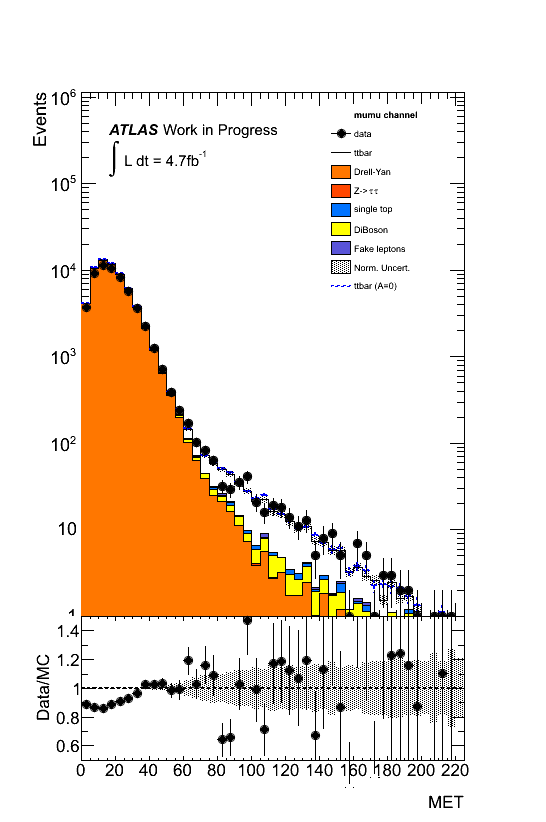
\includegraphics[width=50mm]{f/mumu_control_met_central_double}
%     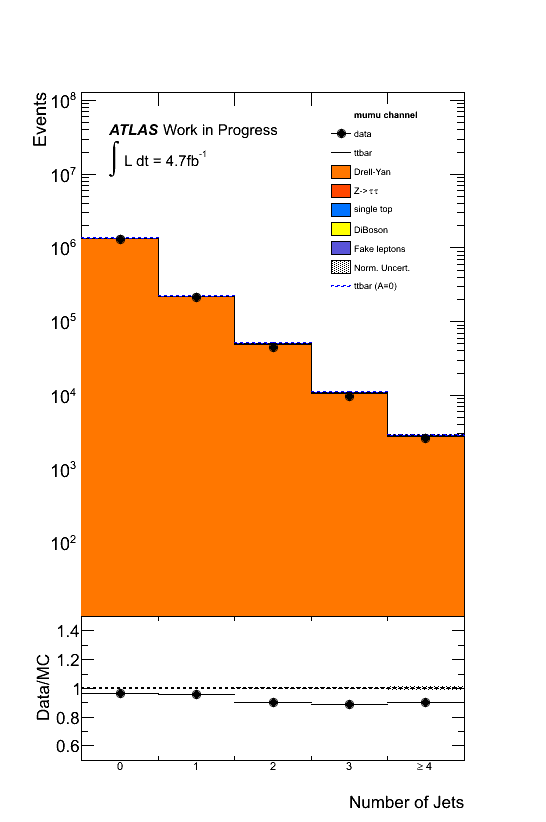
\includegraphics[width=50mm]{f/mumu_control_njet_central_double}
%     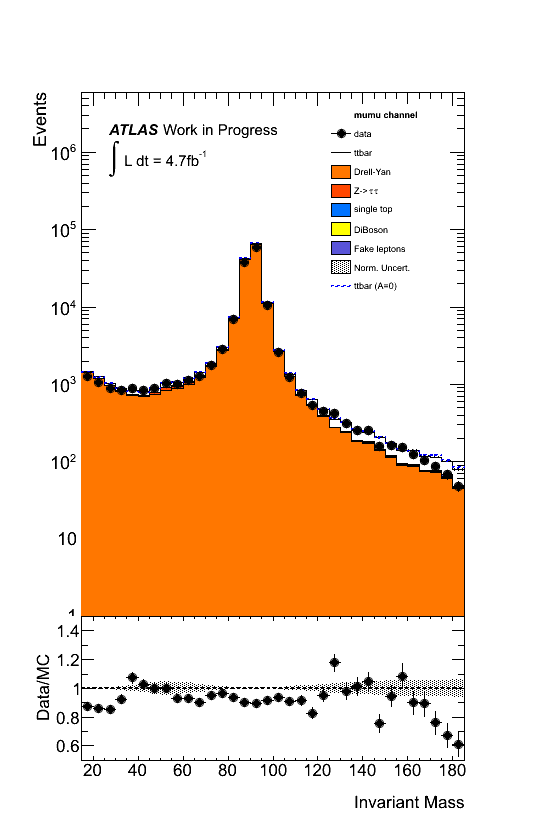
\includegraphics[width=50mm]{f/mumu_control_invmass_central_double}
%     \end{center}
%     \caption{Control plots for the \mumu\ channel.  \etmiss\ distribution in events with a dilepton mass inside the $Z$-boson mass window and at least two jets (left).  The number of jets in events with a dilepton mass inside the $Z$-boson mass window and \etmiss\ $< 40$~GeV (centre) and the invariant mass of opposite-sign lepton pairs in events with at least two jets and with \etmiss\ $< 40$~GeV (right).}
 %    \label{fig:dilep_control_mumu}
 %   \end{figure}

%\begin{figure}[htbp!]
%	\begin{center}
%	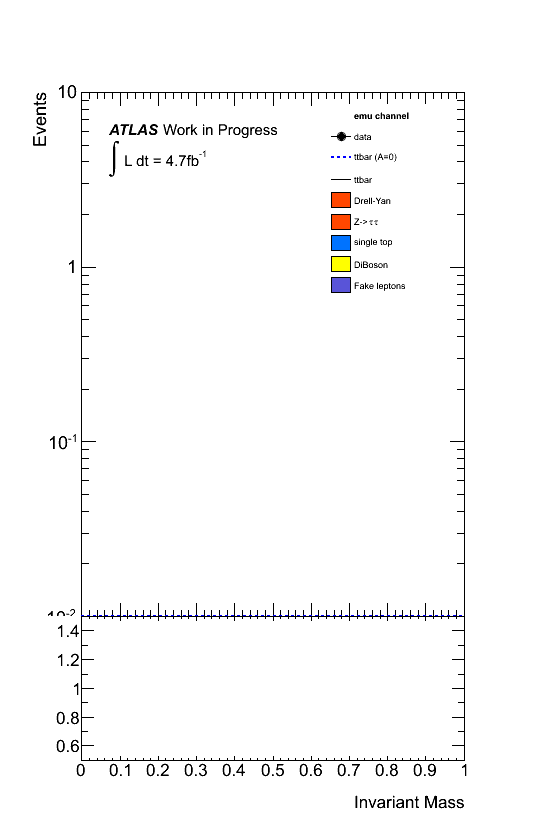
\includegraphics[width=50mm]{f/emu_control_invmass_central_double}
%	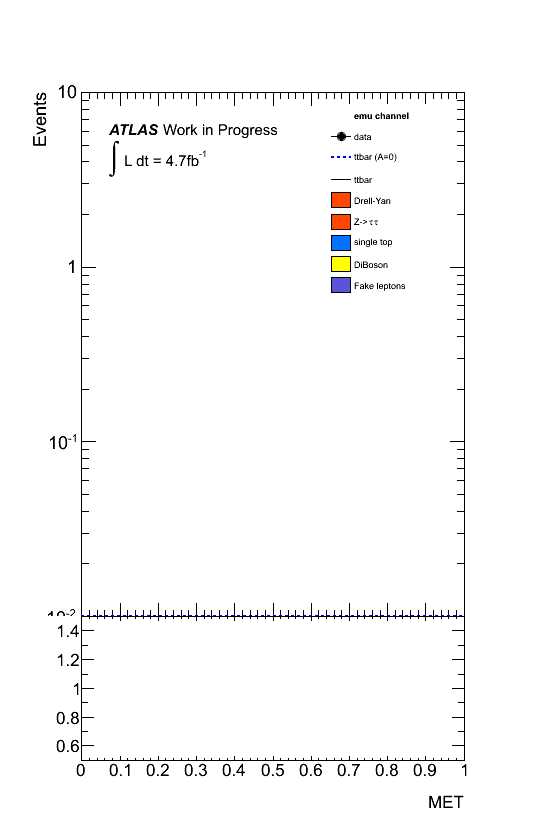
\includegraphics[width=50mm]{f/emu_control_met_central_double}     
%	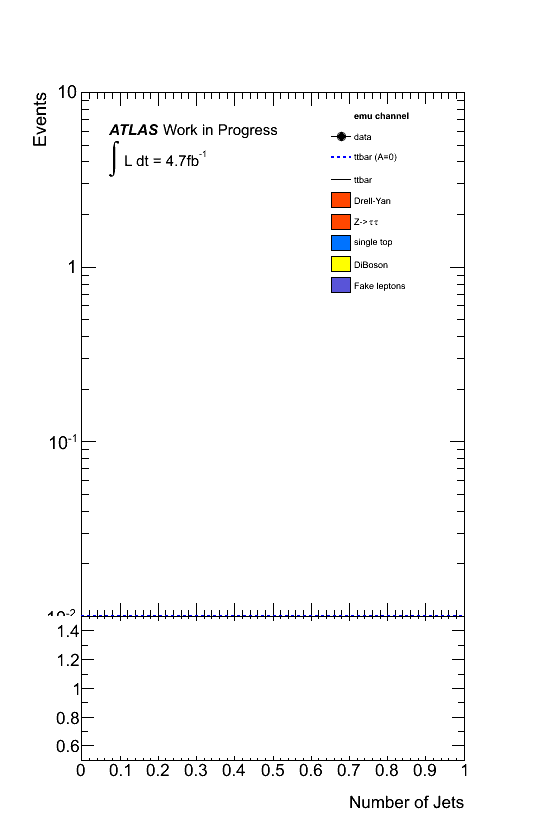
\includegraphics[width=50mm]{f/emu_control_njet_central_double}
%	\end{center}
%	\caption{Control distributions for the \emu\ channel. The invariant mass distribution of the electron and muon (left), the \etmiss\ distribution and the jet multiplicity distribution}
%	\label{fig:dilep_control_emu}
%\end{figure}

\begin{figure}[htbp!]
     \begin{center}
     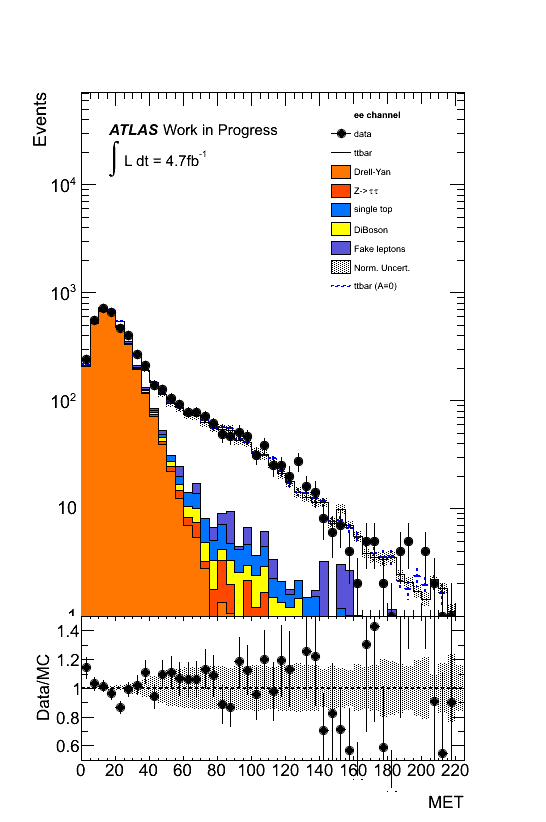
\includegraphics[width=50mm]{f/ee_control_sig_met_central_double}
     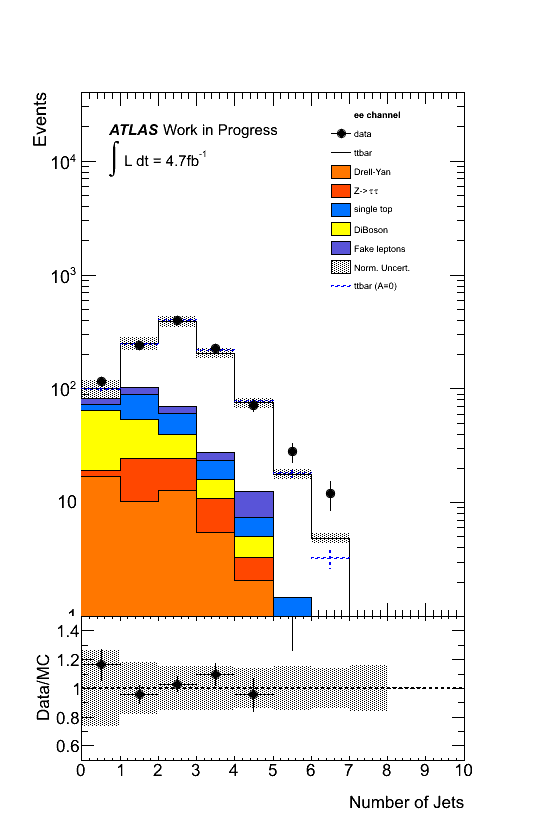
\includegraphics[width=50mm]{f/ee_control_sig_njet_central_double}
     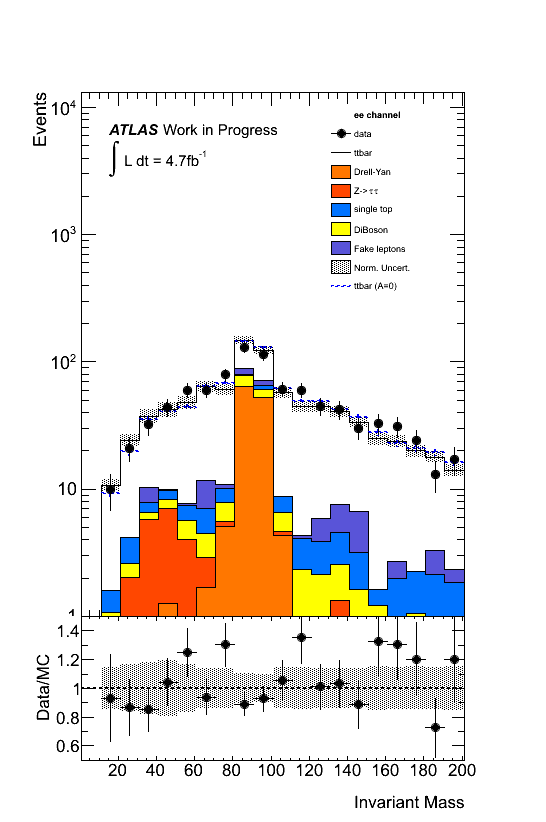
\includegraphics[width=50mm]{f/ee_inv_mass_central_double}
     \end{center}
     \caption{Simulation compared to data in the signal region for the \ee\ channel. The distributions for \etmiss\ , jet multiplicity and invariant mass are shown \emph{left}, \emph{centre} and \emph{right} respectively. In each distribution all selection cuts detailed in section \ref{sec:event_selection} are applied with the exception of the cut applied to the distribution shown.}
     \label{fig:dilep_control_sig_ee}
    \end{figure}

\begin{figure}[htbp!]
     \begin{center}
     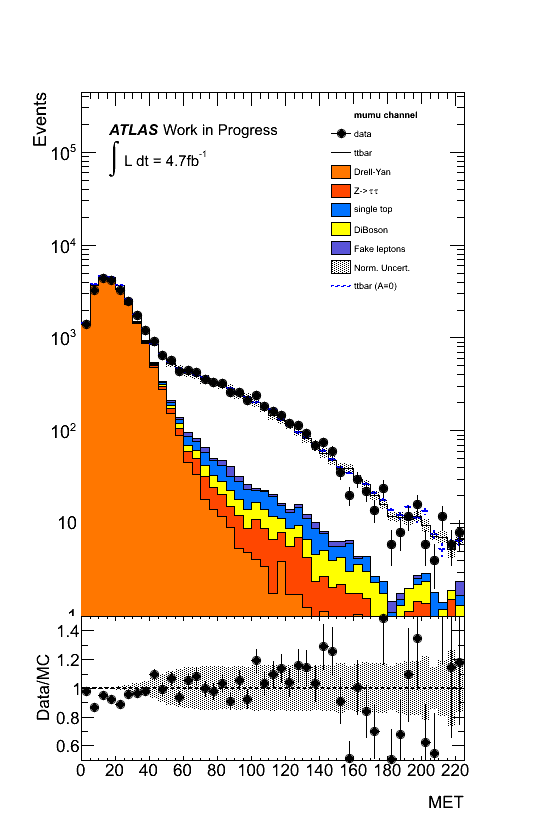
\includegraphics[width=50mm]{f/mumu_control_sig_met_central_double}
     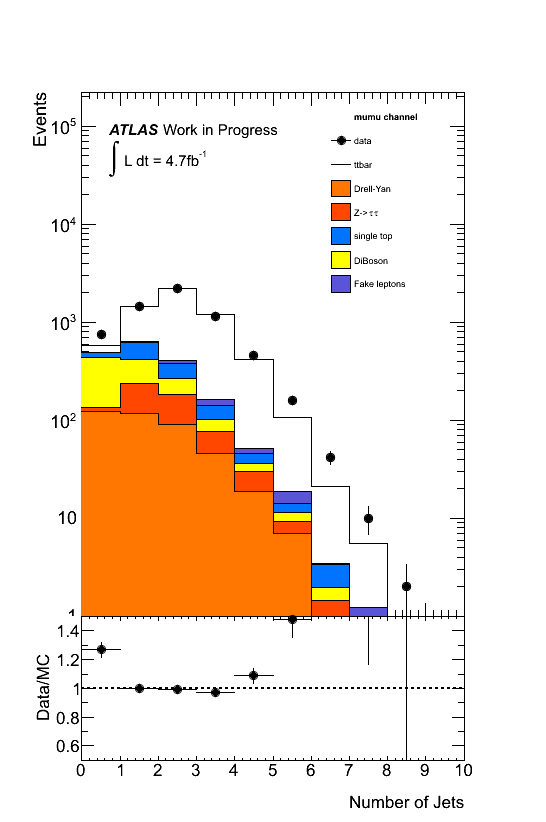
\includegraphics[width=50mm]{f/mumu_control_sig_njet_central_double}
     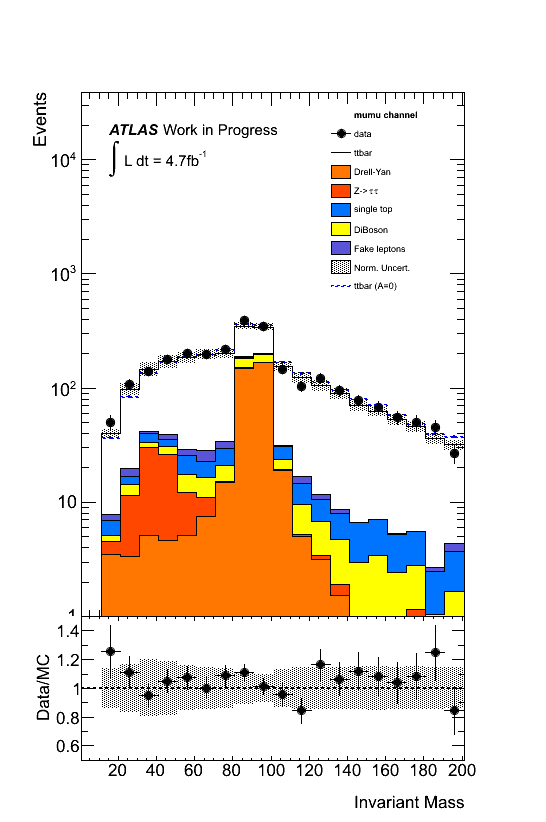
\includegraphics[width=50mm]{f/mumu_inv_mass_central_double}
     \end{center}
     \caption{Simulation compared to data in the signal region for the \mumu\ channel. The distributions for \etmiss\ , jet multiplicity and invraiant mass are shown \emph{left}, \emph{centre} and \emph{right} respectively. In each distribution all selection cuts detailed in section \ref{sec:event_selection} are applied with the exception of the cut applied to the distribution shown.}
     \label{fig:dilep_control_sig_mumu}
    \end{figure}

\begin{figure}[htbp!]
     \begin{center}
     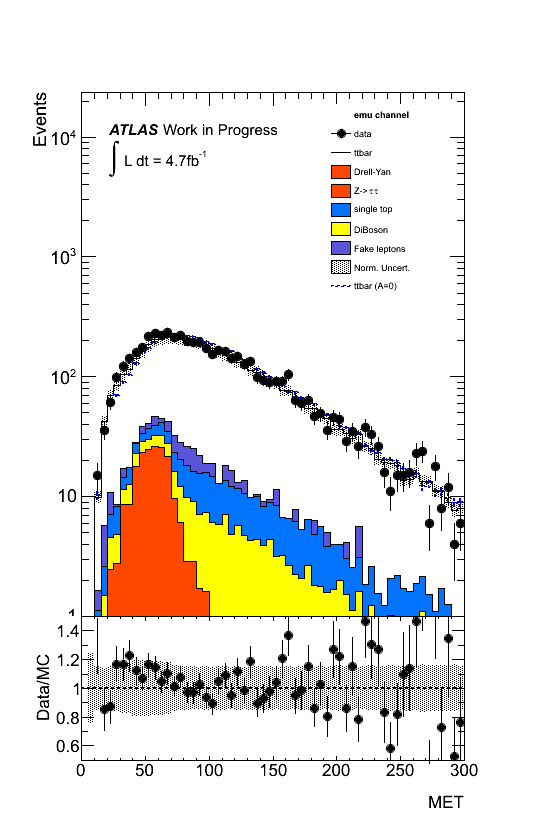
\includegraphics[width=50mm]{f/emu_control_sig_met_central_double}
     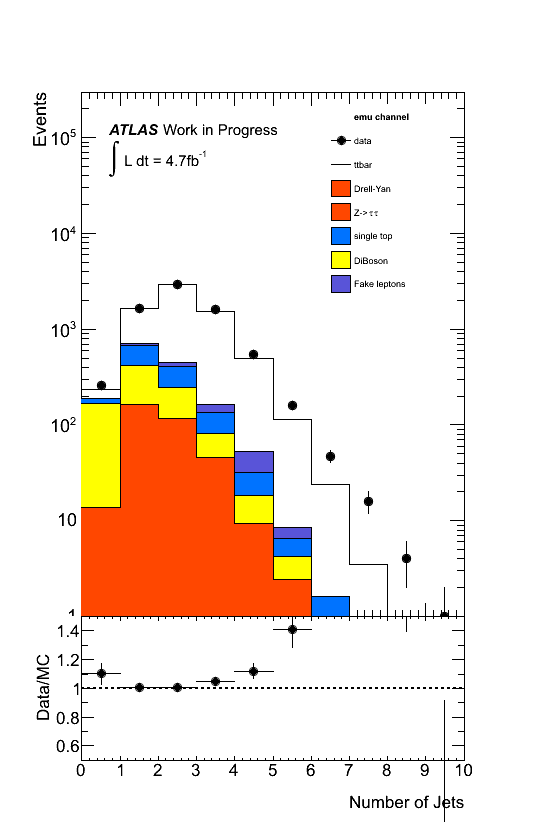
\includegraphics[width=50mm]{f/emu_control_sig_njet_central_double}
     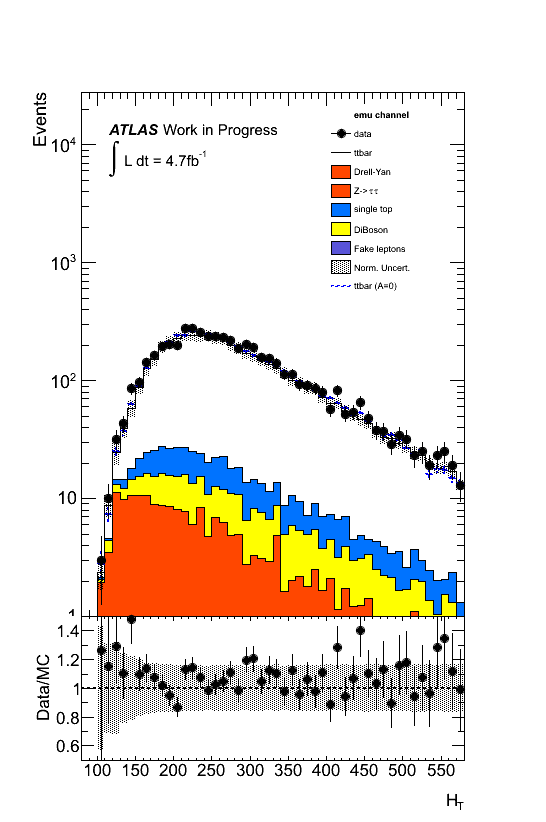
\includegraphics[width=50mm]{f/emu_control_sig_ht_central_double}
     \end{center}
     \caption{Simulation compared to data in the signal region for the \emu\ channel. The distributions for \etmiss\ , jet multiplicity and $H_T$ are shown \emph{left}, \emph{centre} and \emph{right} respectively. In each distribution all selection cuts detailed in section \ref{sec:event_selection} are applied with the exception of the cut applied to the distribution shown.}
     \label{fig:dilep_control_sig_emu}
    \end{figure}

\begin{figure}[htbp!]
     \begin{center}
     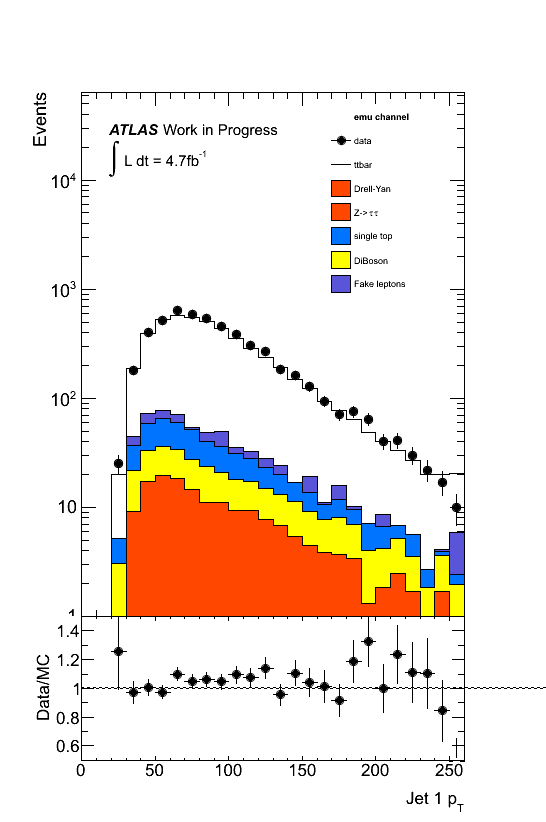
\includegraphics[width=50mm]{f/emu_jet1_pt_central_double}
     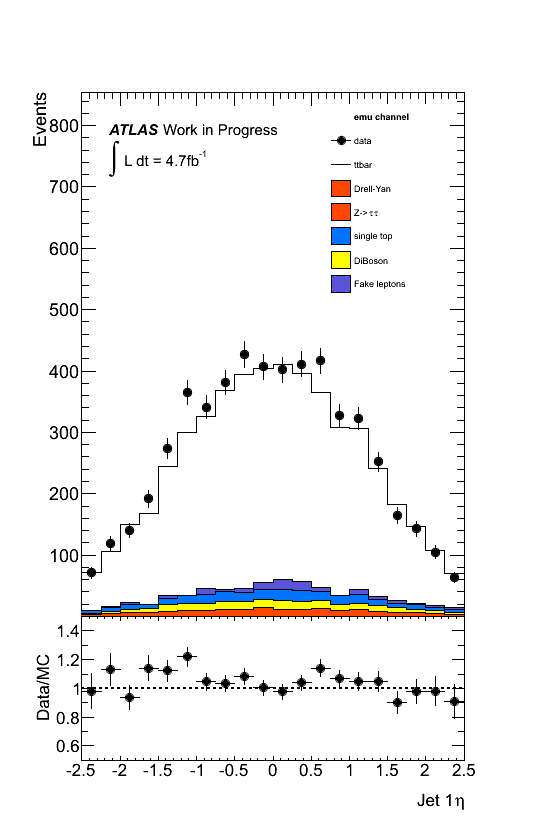
\includegraphics[width=50mm]{f/emu_jet1_eta_central_double}
     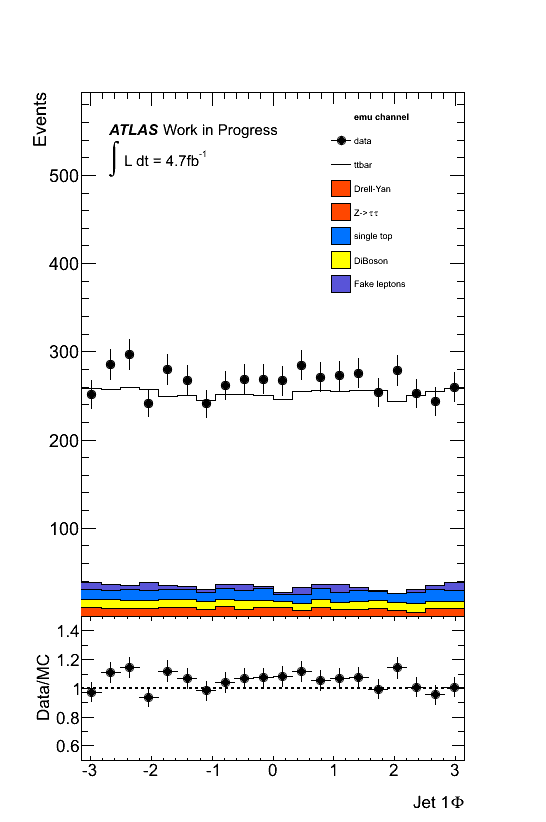
\includegraphics[width=50mm]{f/emu_jet1_phi_central_double}
     \end{center}
     \caption{Distribution of the leading jet \pt\ ,$\eta$, and $\phi$ distributions in the \emu\ channel.}
     \label{fig:dilep_jet1_emu}
    \end{figure}

\begin{figure}[htbp!]
     \begin{center}
     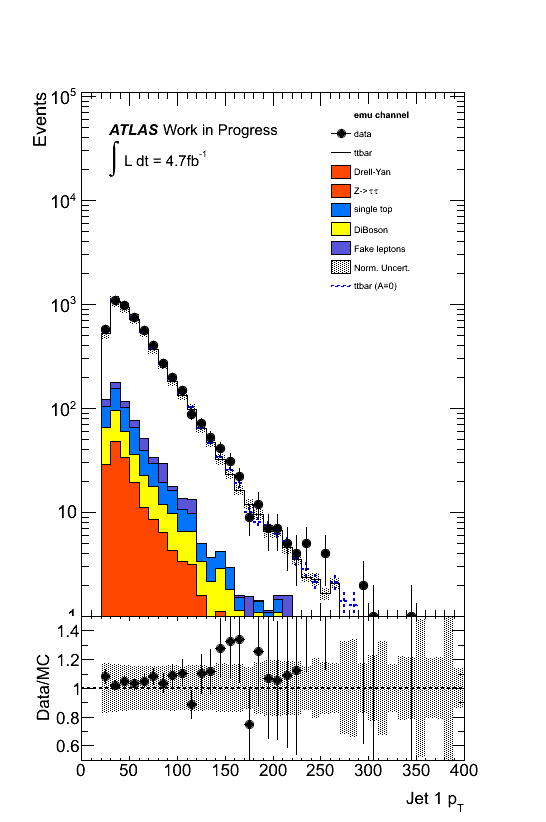
\includegraphics[width=50mm]{f/emu_jet2_pt_central_double}
     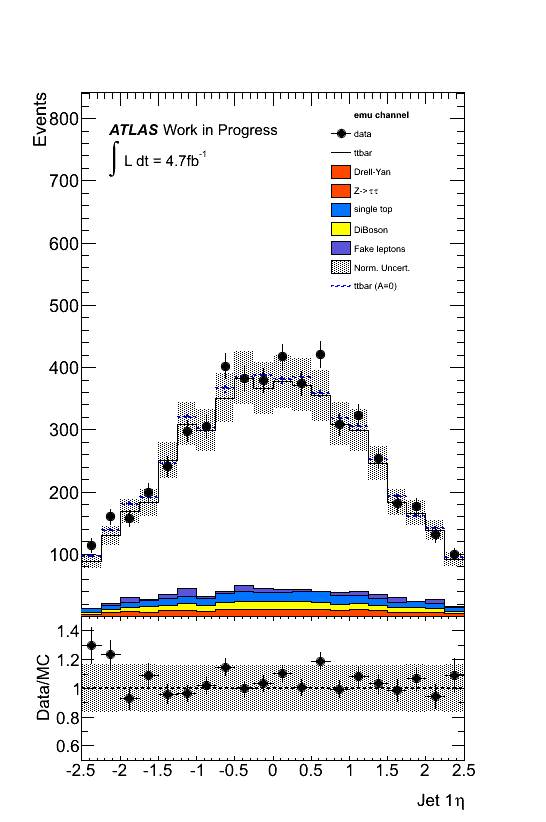
\includegraphics[width=50mm]{f/emu_jet2_eta_central_double}
     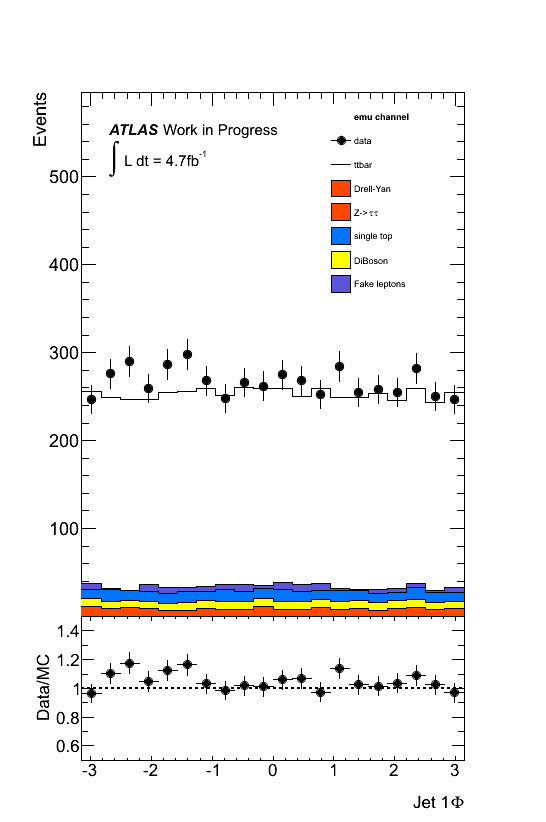
\includegraphics[width=50mm]{f/emu_jet2_phi_central_double}
     \end{center}
     \caption{Distribution of the leading jet \pt\ ,$\eta$, and $\phi$ distributions in the \emu\ channel.}
     \label{fig:dilep_jet2_emu}
    \end{figure}

\begin{figure}[htbp!]
     \begin{center}
     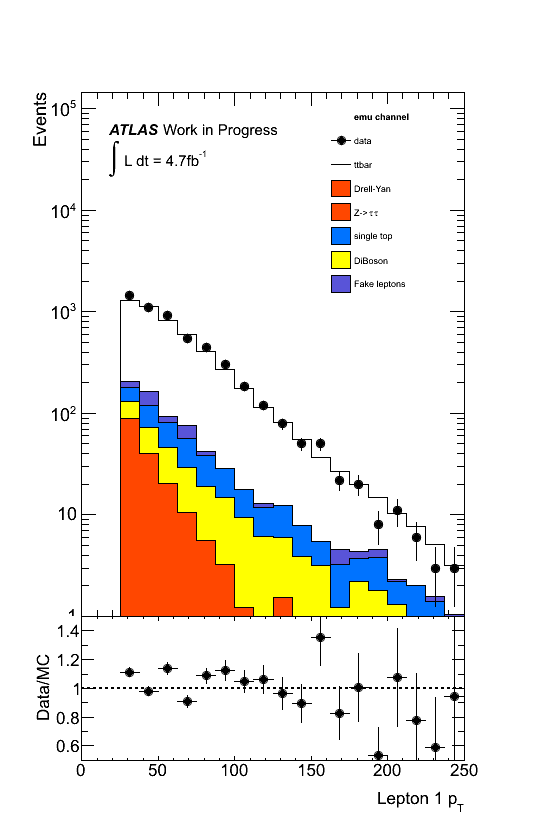
\includegraphics[width=50mm]{f/emu_lep1_pt_central_double}
     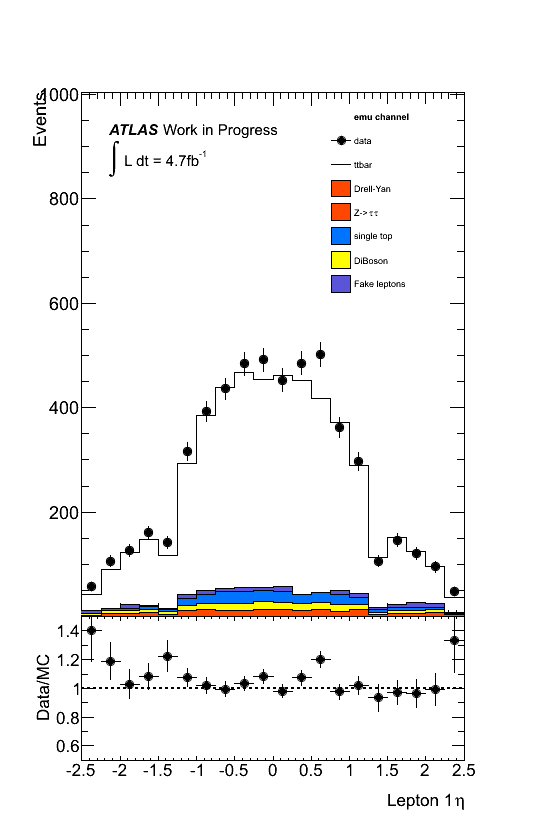
\includegraphics[width=50mm]{f/emu_lep1_eta_central_double}
     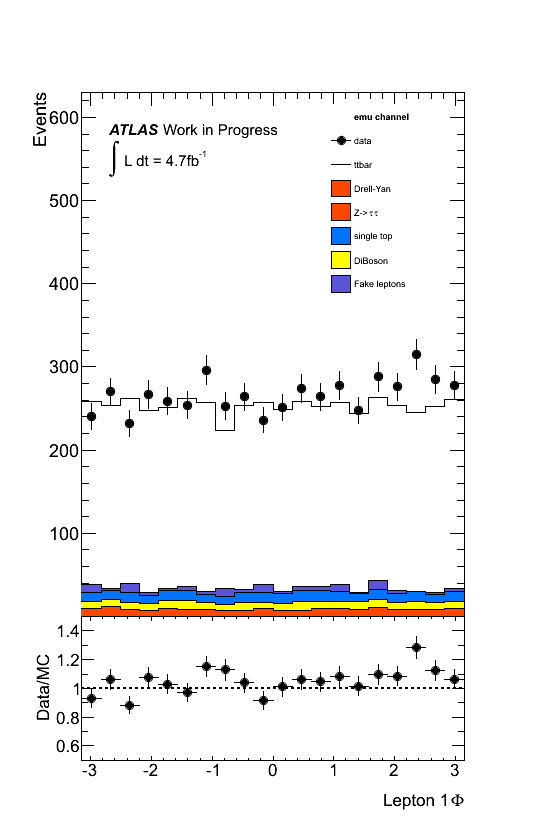
\includegraphics[width=50mm]{f/emu_lep1_phi_central_double}
     \end{center}
     \caption{Distribution of the electron \pt\ ,$\eta$, and $\phi$ distributions in the \emu\ channel.}
     \label{fig:dilep_lep1_emu}
    \end{figure}

\begin{figure}[htbp!]
     \begin{center}
     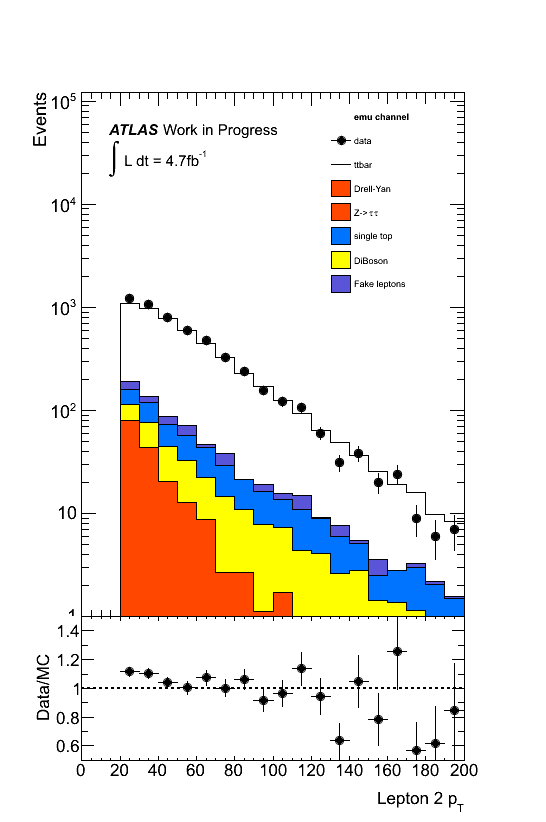
\includegraphics[width=50mm]{f/emu_lep2_pt_central_double}
     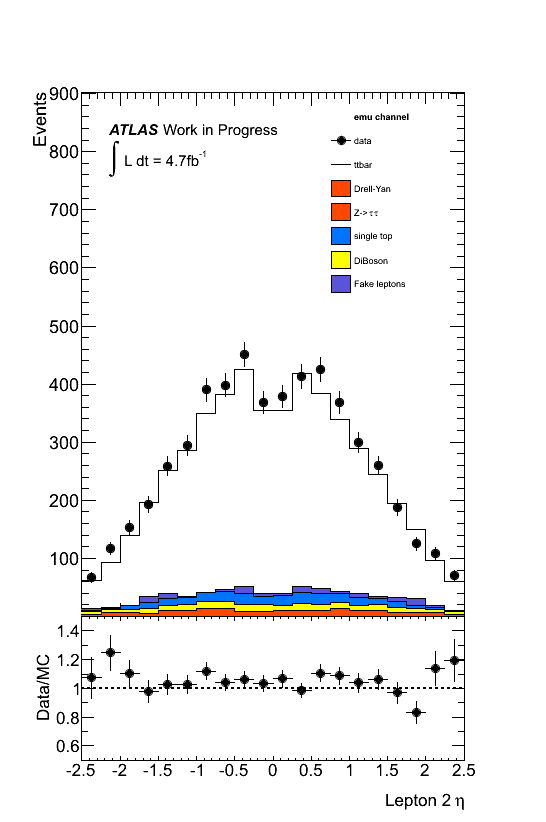
\includegraphics[width=50mm]{f/emu_lep2_eta_central_double}
     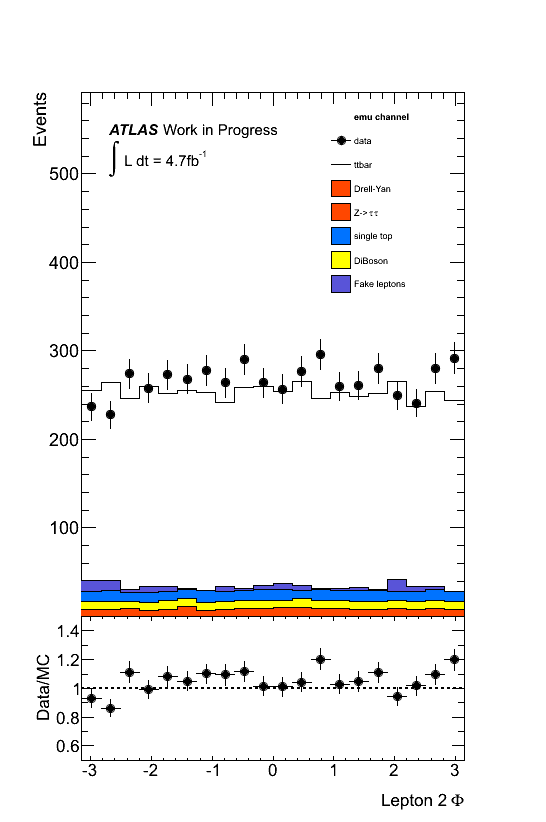
\includegraphics[width=50mm]{f/emu_lep2_phi_central_double}
     \end{center}
     \caption{Distribution of the muon \pt\ ,$\eta$, and $\phi$ distributions in the \emu\ channel.}
     \label{fig:dilep_lep2_emu}
    \end{figure}

\clearpage

\section{Full kinematic reconstruction}
Dilepton \ttbar\ events contain neutrinos. These neutrinos do not interact with the detector so we infer their presence by missing energy in the event. We can only measure this quantity in the transverse direction, \etmiss, and the neutrino's momentum in the z direction must be derived by other means. In the dilepton channel there are two neutrinos but only one measurement for the sum of their transverse momenta, leading to an under-constrained system. Many techniques have been developed to deal with this problem, we describe one of these methods used for this analysis in the following section.

\subsection{Neutrino Weighting}

Neutrino weighting is a reconstruction technique designed to resolve ambiguities inherent to \ttbar\ events with two neutrinos in the final state. It provides the user with reconstructed top quark and neutrino kinematics and limited background rejection\footnote{Though not designed to reject background events, typically the reconstruction does not perform well on non-ttbar events and so a small amount of background event rejection is inherent to the method.}. 

One may define a number of kinematic constraints on properties of the \ttbar\ system using known values and assumptions, and use this solve the under-constrained system (full derivation included in Appendix A). The dilepton final state has twelve observable quantities relevant to reconstruction; the reconstructed momenta of the charged leptons and $b$ quark jets. We can also experimentally measure the combined transverse component of the neutrino momenta, however as we shall see this is not used directly to solve the system. Further constraints may be applied by requiring that the two lepton-neutrino pairs combine to give the $W$ boson mass, and that the $W$ boson, $b$-jet pairs combine to give the top mass. Even using all of these quantities, the system is still unconstrained. We can introduce an additional two parameters, the pseudo-rapidities of the un-observed neutrinos, that allows us to fully constrain the system. These pseudo-rapidities ($\eta_1\eta_2$) cannot be measured experimentally, and so we assign them random values. In other methods the \etmiss\ is used to inform this assumption, however this is not the case for neutrino weighting. A random choice for $\eta_1\eta_2$ is unlikely to be correct so we must inform this choice as much as possible.
      
      \begin{figure}[h!]
      \begin{center}
     
      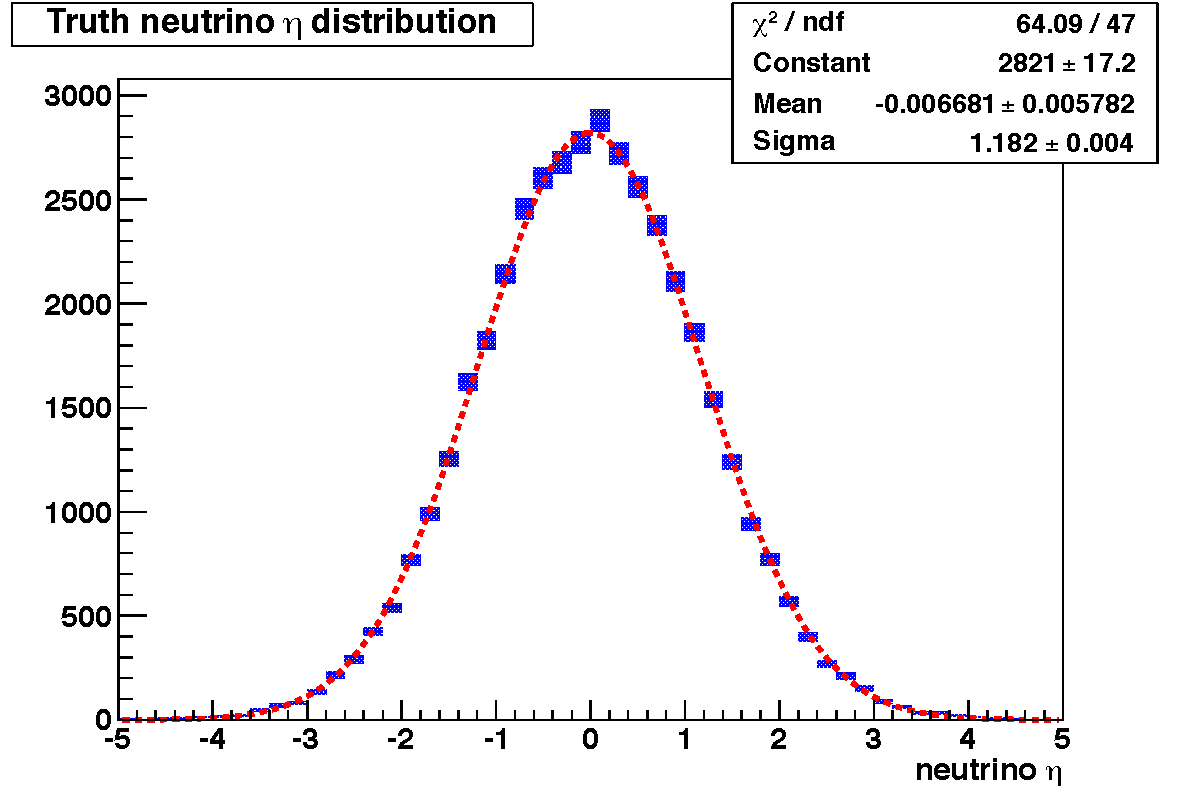
\includegraphics[width=75mm]{f/truth_neutrino_eta}
     
      \caption{Distribution of neutrino pseudo-rapidities in MC@NLO (left) and comparison between neutrino $\eta$ distribution in events with standard model spin correlation and no spin correlation (right)}
      \label{fig:nu_dist}
      \end{center}
      \end{figure}

\todo[inline]{plot showing that neutrino eta distribution is the same for spin and nospin}
     
      From Monte-Carlo we can see that the neutrino pseudo-rapidities are well defined as a Gaussian distribution with mean of zero and unit width (Figure \ref{fig:nu_dist}). These distributions are also found to be independent of spin correlation. We perform the reconstruction many times for many different assumptions of neutrino $\eta$. Each event a random $\eta$ is generated for each neutrino using the Gaussian distribution derived from Monte Carlo in the range $-4.0 < \eta < 4.0$. This procedure is repeated 50 times per event and was found to be more effective than previous methods of performing a linear scan of fixed points \cite{Meyer:2007zz}. 

Using the now constrained system the number of solutions per neutrino assumption is 8; two from the ambiguity of the lepton-jet pairing and four (per pairing) from the quadratic terms in the neutrino solution (see Appendix equation XX). The assumption is performed 50 times per neutrino $\eta_i$ assumption, totalling 400 solutions per event.
     
So far we have not used the measured \etmiss\ in the reconstruction, and we have obtained 400 solutions with no information on which is the correct solution, or rather the solution which most accurately reflects the true neutrino four vectors. We can now use the \etmiss\ as a way to weight each solution, based on how well the reconstructed neutrinos agree with the observed \etmiss\ . The function used to calculate this weight is shown in equation \ref{eq:weight}, where $\sigmet$ is the resolution of the $x$ or $y$ component of missing transverse energy~\cite{nuWtmass}. The resolution is the same for the $x$ and $y$ direction.

\begin{equation}
    w=\sum_{\eta_{1},\eta_{2}}\sum_{solutions}    
    \exp\left(-\frac{\left(\metx^{calc}-\metx^{obs} \right)^{2}}{2\sigmet} \right)
    \exp\left(-\frac{\left(\mety^{calc}-\mety^{obs} \right)^{2}}{2\sigmet}
    \right)
    \label{eq:weight}
    \end{equation}
     
The final neutrino four momenta may be selected in one of two ways. Either the solution with the highest weight may be chosen, or the weighted sum of all solutions may be taken; the later typically produces better performance. Occasionally an incorrect lepton-jet pairing can give a very high weight whereas in the weighted average this effect is usually mitigated by the combined weights of more accurate solutions.
     
\begin{figure}[htbp!]
	\begin{center}
	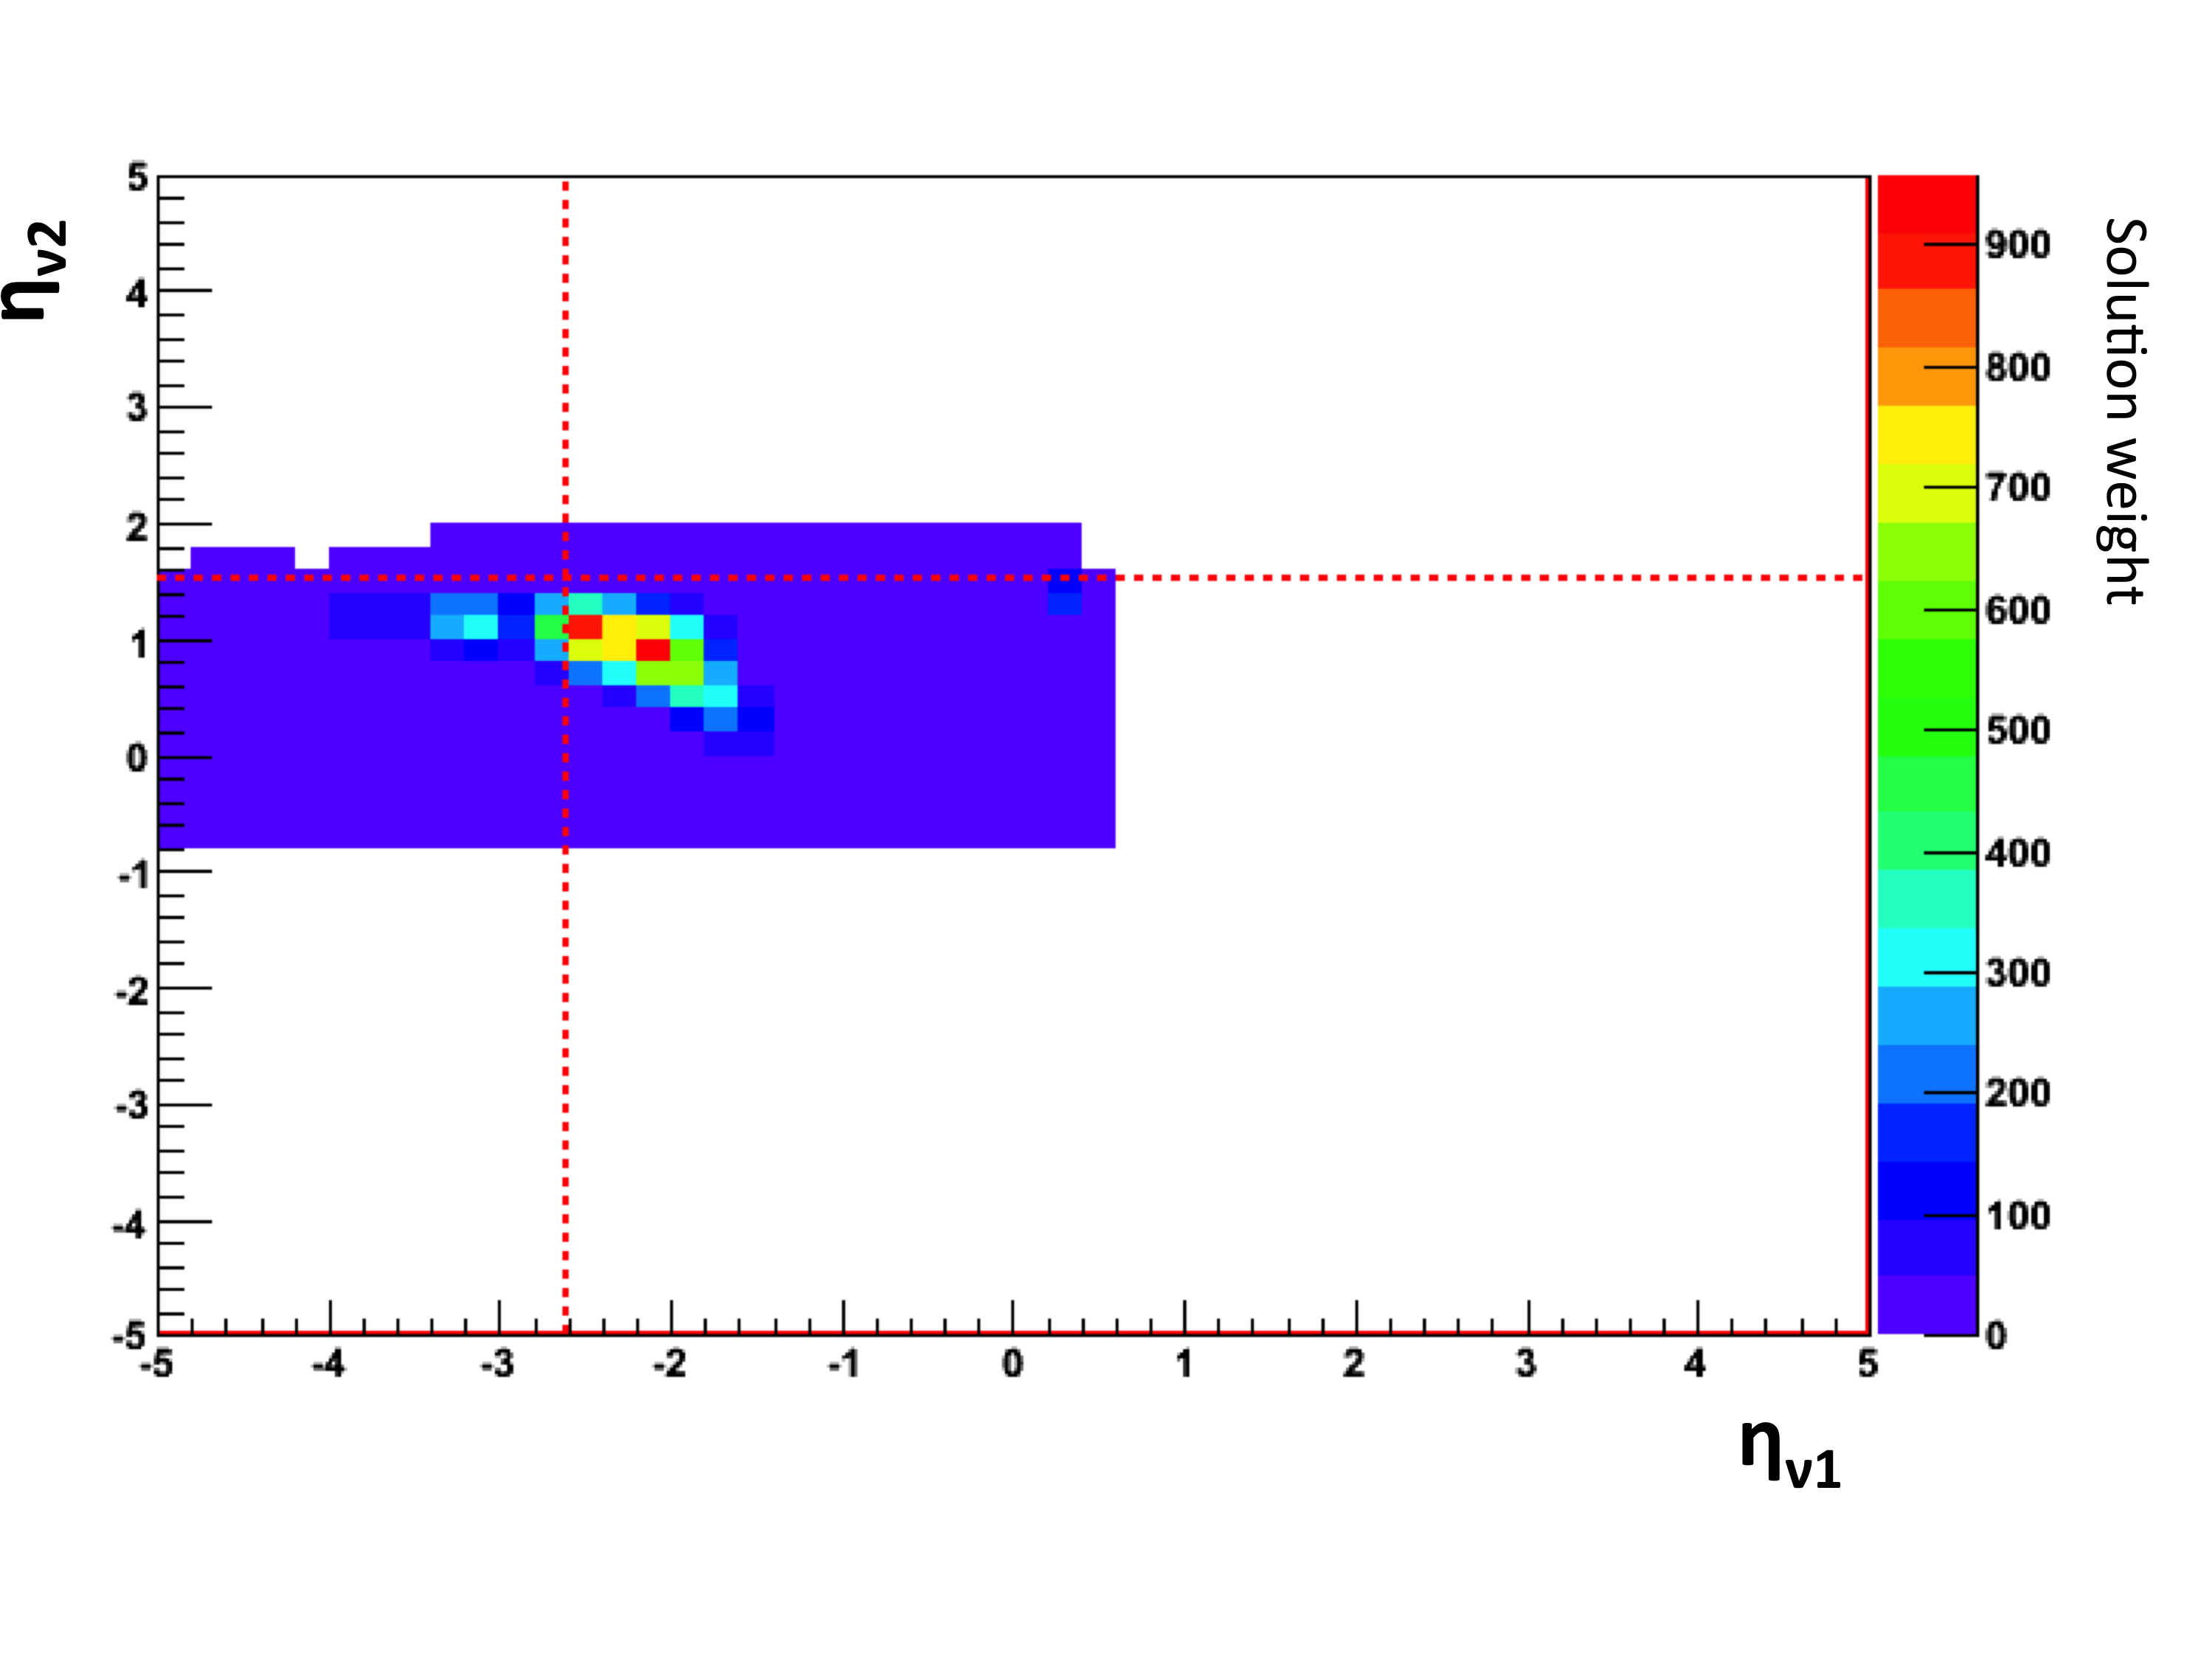
\includegraphics[width=75mm]{f/top_nuweights_1d_2}
	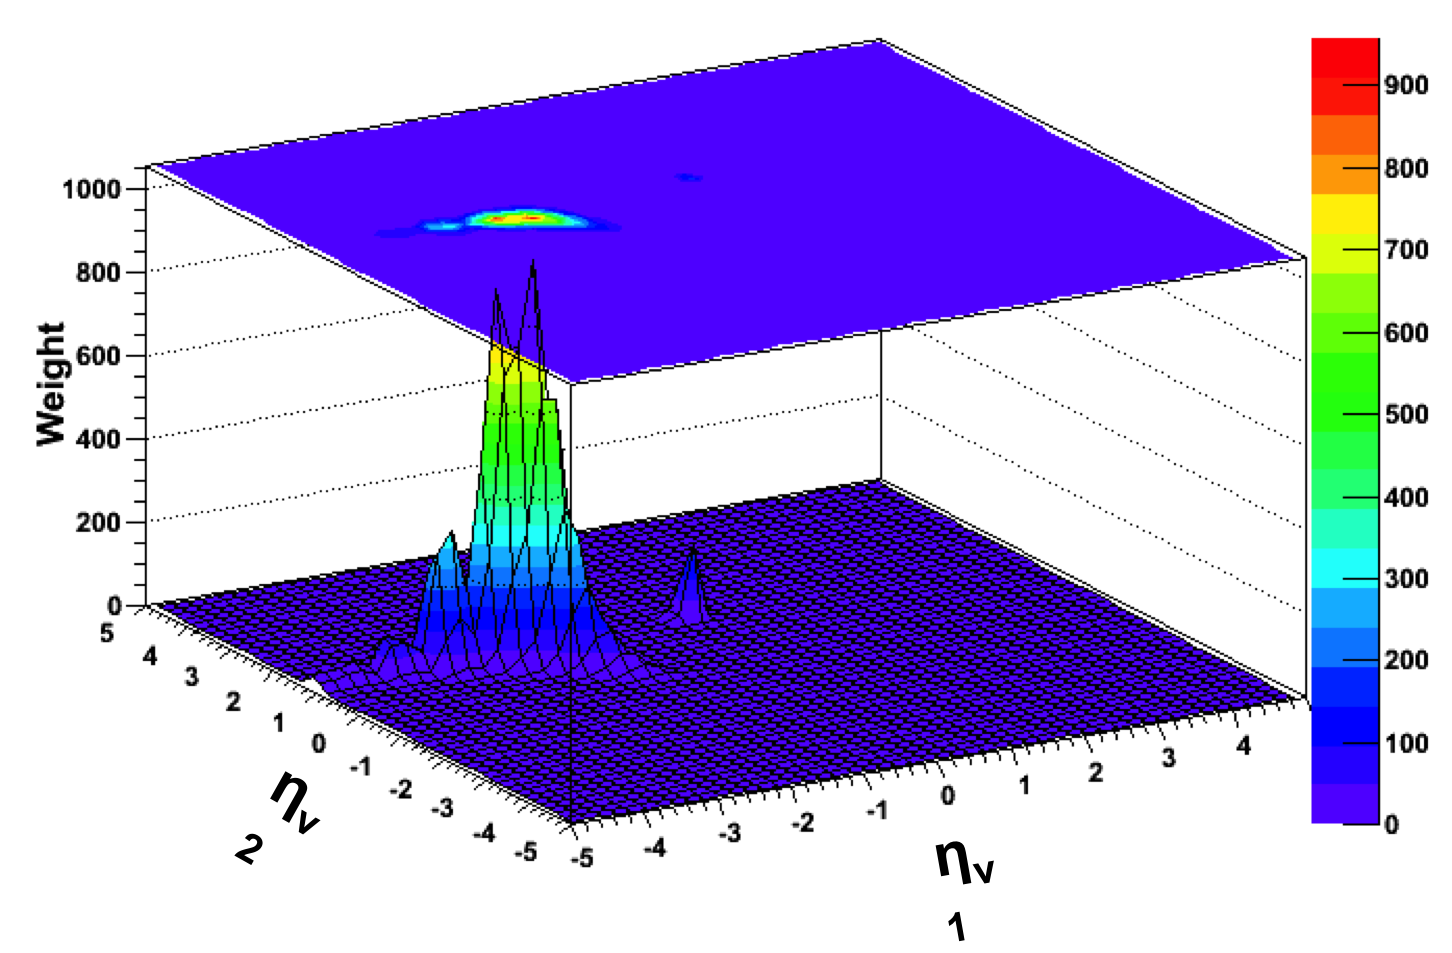
\includegraphics[width=75mm]{f/top_nuweights_2d_2}
	\end{center}
	\caption{Weight distributions for neutrino weighting solutions for a single event. True values for the neutrino $\eta$ are indicated with the red dashed lines.}
	\label{fig:top_nuweights}
\end{figure}

Jet measurements at ATLAS can provide useful information on the underlying parton that seeded them (in this case the b quarks from the top quark decays) however their observed physical quantities, such as energy and direction, are never exactly the same as that of the underlying parton. To account for this, the jet energies are smeared many times for each assumption of $\eta_1\eta_2$ within the measured energy resolution of the jet. The same could be considered for leptons, but at ATLAS the lepton energy resolution is orders of magnitude smaller than the jet energy resolution and hence this is not considered. This was not the case at previous colliders using neutrino weighting (such as D0) and is only applicable to detectors such as ATLAS, where lepton energy resolution is very good.

\todo[inline]{Find references for the Jet Energy Resolution paper, maybe show the resolution as a function of jet pt}

\subsection{Topology and KLFitter}
Two other reconstruction algorithms are investigated. KLFitter\footnote{There are two implementations of this algorithm, one for dilepton \ttbar\ events and one for semi leptonic \ttbar events. Only the dilepton version is discussed.} is a Kinematic Likelihood Fitter that uses the same numeric solution as neutrino weighting but instead of using a weighting function, uses a likelihood function to qualify solutions. In addition the uncertainty on the b-quark energy is implemented in the likelihood via transfer functions, rather than using energy smearing~\cite{klfitter}.

Topology use the \etmiss\ in the reconstruction directly, using the same constraints as neutrino weighting, leading to only 8 possible solutions per event. The best is chosen using a chi-squared technique~\cite{topology}.

Both algorithms utilise information not available in neutrino weighting, the invariant mass of the lepton and b-jet pair. This is useful in removing the lepton-jet pair ambiguity but effectively removes the possibility of considering more than 2 jets in the event for the reconstruction. This will be discussed further in section \ref{sec:reco_comparison}.

\todo[inline]{References for other reconstruction methods}

\clearpage

\begin{figure}[htbp!]
	\begin{center}
	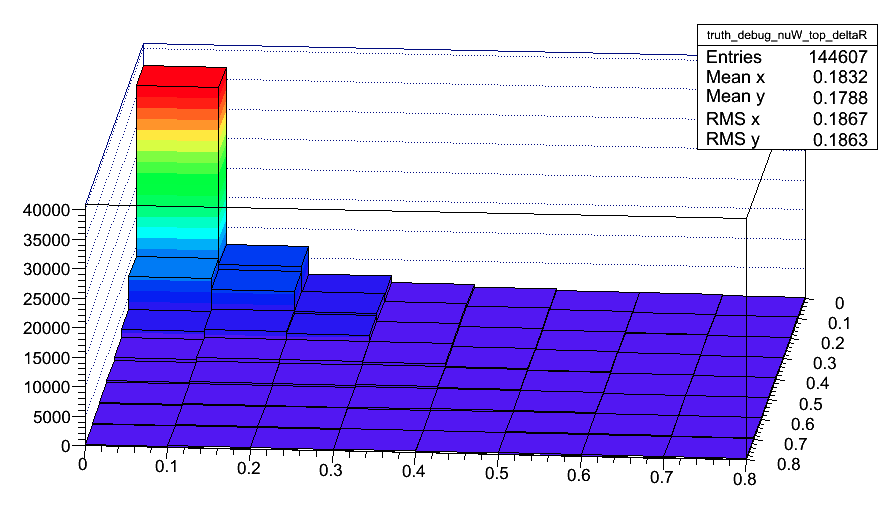
\includegraphics[width=100mm]{f/top_deltaR}
	\end{center}
	\caption{Distance in $\eta - \phi$ space of the reconstructed top to the truth top (x-axis) and the reconstructed anti-top to the true anti-top (y-axis) as a function of absolute number of events.}
	\label{fig:top_dr}
\end{figure}

\subsection{Efficiency}
Three reconstruction algorithms have been discussed in detail (though more exist). In order to compare the advantages and disadvantages of each reconstruction method we define a set of parameters common to each. The parameters are expressed as efficiencies based on the how well the reconstructed particles describe the underlying truth particles in the Monte Carlo. We can use these efficiencies to categorise events where the reconstruction describes the underlying truth information well (matched) and events where the reconstruction did not describe the truth information (unmatched). In this analysis it is the direction of the top quarks that is the most crucial reconstructed quantity and we categorise the events based on how well the top directions are described by the reconstruction. We define the variable $\Delta R (t\bar{t})$ to be the distance in $\eta - \phi$ space of the weighted average \ttbar\ four vectors and the true four vectors in the MC. If this value is less than 0.4 for both the reconstructed top and reconstructed anti-top we say that the event is ``matched" and if not we say that it is ``un-matched". The value of 0.4 is arbitrary since the purpose is not to measure a predictable physical quantity but rather to define a variable with which to compare different reconstruction methods in a consistent way. An example of this variable is shown in figure \ref{fig:top_dr}.


The efficiencies are measured using the nominal \ttbar\ MC@NLO sample and are presented as a fraction of the untagged dilepton selection (total events) and as a fraction of events with at least one solution (solved events). The efficiencies are independent of spin correlation and agree in both MC@NLO samples within the statistical uncertainties. The efficiencies for four cases are shown in table \ref{tab:nu_comparison}. For a selection inclusive of all jets, neutrino weighting had the highest reconstruction efficiency and the highest matched efficiency. KLFitter could not be considered in this selection due to technical limitations of the algorithm and it should be noted that the Topology algorithm was not designed to be used in such a selection. For a selection that include two b-tagged jets (or 1 b-tagged and one high $p_T$ jet) KLFitter has the highest reconstruction efficiency and topology has the highest matched efficiency. The implications of using a b-tagged selection render this unsuitable for this analysis. The reasons for this are described in detail in section \ref{sec:btagged_selection}.
%\vspace{10mm}
\begin{table}[htbp!]
\begin{center}
\footnotesize
%	\begin{tabular}{  c  c  c  c  }
%	\multicolumn{4}{l}{\textbf{ALL JETS}} \\
%	\hline
%	\textbf{Efficiency}       & \textbf{NuW} & \textbf{NuW Mass} & \textbf{Topo} \\
%	\hline
%	\multicolumn{4}{c}{ \textbf{Total events} } \\
%	Reco Eff                  & 96.0 & 96.8 & 82.3 \\
%	$\Delta R(t\bar{t})<0.4$  & 28.5 & 28.5 & 16.1 \\
%	$\Delta R(t\bar{t})<0.2$  & 11.3 & 11.7 &  6.8 \\
%	\hline
%	\multicolumn{4}{c}{ \textbf{Solved events} } \\
%	$\Delta R(t\bar{t})<0.4$  & 29.7 & 29.5 & 19.6 \\
%	$\Delta R(t\bar{t})<0.2$  & 11.8 & 12.1 &  8.3 \\	
%	\hline
 %   \end{tabular}
%    \quad
 %   \begin{tabular}{ c c c c }
	%\multicolumn{4}{l}{\textbf{B-TAGGED}} \\
%	\hline
%	\textbf{Efficiency}       & \textbf{NuW} & \textbf{Topo} & \textbf{KLfitter*} \\
%	\hline
 %   \multicolumn{4}{c}{ \textbf{Total events} }    \\
%	Reco Eff                  & 62.8 & 66.7 & 70.0 \\
%	$\Delta R(t\bar{t})<0.4$  & 18.3 & 26.5 & 22.0 \\
%	$\Delta R(t\bar{t})<0.2$  &  8.9 & 11.2 &      \\
%	\hline
 %   \multicolumn{4}{c}{ \textbf{Solved events} }   \\
%	$\Delta R(t\bar{t})<0.4$  & 29.1 & 39.7 & 31.4 \\
%	$\Delta R(t\bar{t})<0.2$  & 14.1 & 16.8 &      \\	
%	\hline	
%	\end{tabular}
%	\end{center}
%	\caption{Table of Neutrino weighting (NuW) and Topology (Topo) reconstruction efficiency. Two cases are shown, the case for an inclusive selection and for a double b-tagged selection (where events with only one b-tagged jet are included and the second jet is the highest \pt\ non b-tagged jet). The case where the top mass constraint is flucutated in NuW is also shown. \\ \\ \footnotesize{*KLfitter numbers were provided by independent analysers on limited statistics and hence has much larger uncertainties than Topo of NuW}}

	\begin{tabular}{  c  c  c  }
	\multicolumn{3}{l}{\textbf{ALL JETS}} \\
	\hline
	\textbf{Efficiency}       & \textbf{NuW} & \textbf{Topo} \\
	\hline
	\multicolumn{3}{c}{ \textbf{Total events} } \\
	Reco Eff                  & 96.0 & 82.3 \\
	$\Delta R(t\bar{t})<0.4$  & 28.5 & 16.1 \\
	$\Delta R(t\bar{t})<0.2$  & 11.3 &  6.8 \\
	\hline
	\multicolumn{3}{c}{ \textbf{Solved events} } \\
	$\Delta R(t\bar{t})<0.4$  & 29.7 & 19.6 \\
	$\Delta R(t\bar{t})<0.2$  & 11.8 &  8.3 \\	
	\hline
   \end{tabular}
    \quad
\quad	
\quad
    \begin{tabular}{ c c c c }
	\multicolumn{4}{l}{\textbf{B-TAGGED}} \\
	\hline
	\textbf{Efficiency}       & \textbf{NuW} & \textbf{Topo} & \textbf{KLfitter*} \\
	\hline
    \multicolumn{4}{c}{ \textbf{Total events} }    \\
	Reco Eff                  & 62.8 & 66.7 & 70.0 \\
	$\Delta R(t\bar{t})<0.4$  & 18.3 & 26.5 & 22.0 \\
	$\Delta R(t\bar{t})<0.2$  &  8.9 & 11.2 &      \\
	\hline
    \multicolumn{4}{c}{ \textbf{Solved events} }   \\
	$\Delta R(t\bar{t})<0.4$  & 29.1 & 39.7 & 31.4 \\
	$\Delta R(t\bar{t})<0.2$  & 14.1 & 16.8 &      \\	
	\hline	
	\end{tabular}
	\end{center}
	\caption{Table of Neutrino weighting (NuW) and Topology (Topo) reconstruction efficiencies in two selections. B-TAGGED is defined as the two highest $p_T$ b-tagged jets or, in the case of only one b-tagged jet in the event, the highest $p_T$ non b-tagged jet is used. \\ \\ \footnotesize{*KLFitter numbers were provided by independent analysers on limited statistics and hence has much larger uncertainties than Topo of NuW}}
\label{tab:nueff}
\end{table}



%\begin{table*}[!h]
%\begin{center}
%\scriptsize
%  \begin{tabular}{ c | c  c | c  c | c  c}
%    \hline
%    \textbf{Efficiency} & \textbf{ee (tot)} & \textbf{ee (rel)} & \textbf{$\mu\mu$ (tot)} & \textbf{$\mu\mu$ (rel)} & \textbf{e$\mu$ (tot)} & \textbf{e$\mu$ (rel)} \\
%    \hline
%    Reconstructed events               & 96.0 &      & ---- &      & ---- &      \\
%    \hline
%    $\Delta R (t\bar{t}) < 0.4$        & 19.7 & 24.2 & 25.4 & 33.1 & 22.7 & 30.3 \\
%    $\Delta R _(t\bar{t}) < 0.2$       &  7.6 &  9.4 & 10.7 & 13.9 &  9.3 & 12.5 \\
%    \hline
%    $\Delta R (\nu\bar{\nu}) < 0.4 $   &  1.9 &  2.3 &  4.7 &  6.1 &  2.5 &  3.3 \\
%    $\Delta R (\nu\bar{\nu}) < 0.2 $   &  0.0 &  0.0 &  0.0 &  0.0 &  2.5 &  3.3 \\
%    \hline
%    Correct Pair                       &      &      &      &      &      &      \\
%    All top correct                    &  8.3 & 10.2 &  8.7 & 11.4 &  7.4 &  9.9 \\
%    \hline
%    \end{tabular}
%  \end{center}
%	\label{tab:nu_eff}
%  \caption{Table showing the efficiencies of the mean weighted reconstruction in ttbar Monte Carlo.}
%\end{table*}

\subsubsection{Performance on signal Monte Carlo}
The efficiencies for neutrino weighing were measured in both the SM sample and the uncorrelated sample. No difference was observed in the reconstruction efficiencies however an interesting effect was observed in distribution shapes. Events with spin correlation included where no truth matching is achived are indistinguishable from uncorrelated events as shown in figure \ref{fig:matching}. This is a useful feature as unmatched events do not distort the shape of the matched events. If the shape of the unmatched events had been somehow anti-correlated with those that matched the overall sensitivity might have been reduced. The conclusion is that poorly reconstructed events simple act as a flat background in the extraction method (described in section \ref{sec:extraction}) and do not detract from the separation of the two hypotheses templates. This result only applied to neutrino weighting and cannot be assumed for other reconstruction methods.

\missingfigure{Plot of unmatched ttbar events}

\subsubsection{Performance on background Monte Carlo}
In principle, the weight distribution may contain information useful for background suppression. Background events should be harder to reconstruct and provide on average lower weights. If one were to cut on the weight distribution magnitude, it may be possible to suppress background. This analysis was formulated to be as inclusive as possible, and relies on good understanding of the background shapes rather than attempting to fully remove them and so this possible feature was not used. A further study could include an investigation into this possibility and would be particularly useful for analyses that wished to perform multi-dimensional unfolding of reconstructed distributions where additional background suppression would be desirable. 

\subsubsection{Comparison with other methods}
\label{sec:reco_comparison}
The Neutrino Weighting algorithm was compared to two other reconstruction algorithms; KLFitter$_{dilepton}$ and Topology. Neither algorithm is capable of considering an inclusive jet selection and so the constraint is made that only two jets are selected with at least one b-tag. In cases where there are more than two b-tags, the two with the highest \pt\ are chosen. A selection where the two jets with the highest b-tag weight were used was also investigated, however the conclusions in both cases remains the same.

Both algorithms give higher efficiency of matched \ttbar\ events than neutrino weighting. This is due to an extra component available in both. The lepton-jet invariant mass distribution is sensitive to correct or incorrect lepton-jet pairings, as shown in figure \ref{fig:lep_jet_mass}. In the simple case of two jets, the difference between the invariant masses tends to be negative for correct pairings. It is not possible to perform this cut in neutrino weighting due to the inclusive jet selection. 
\todo[inline]{Cite the WHelicity paper for this}

\begin{figure}[htbp!]
     \begin{center}
     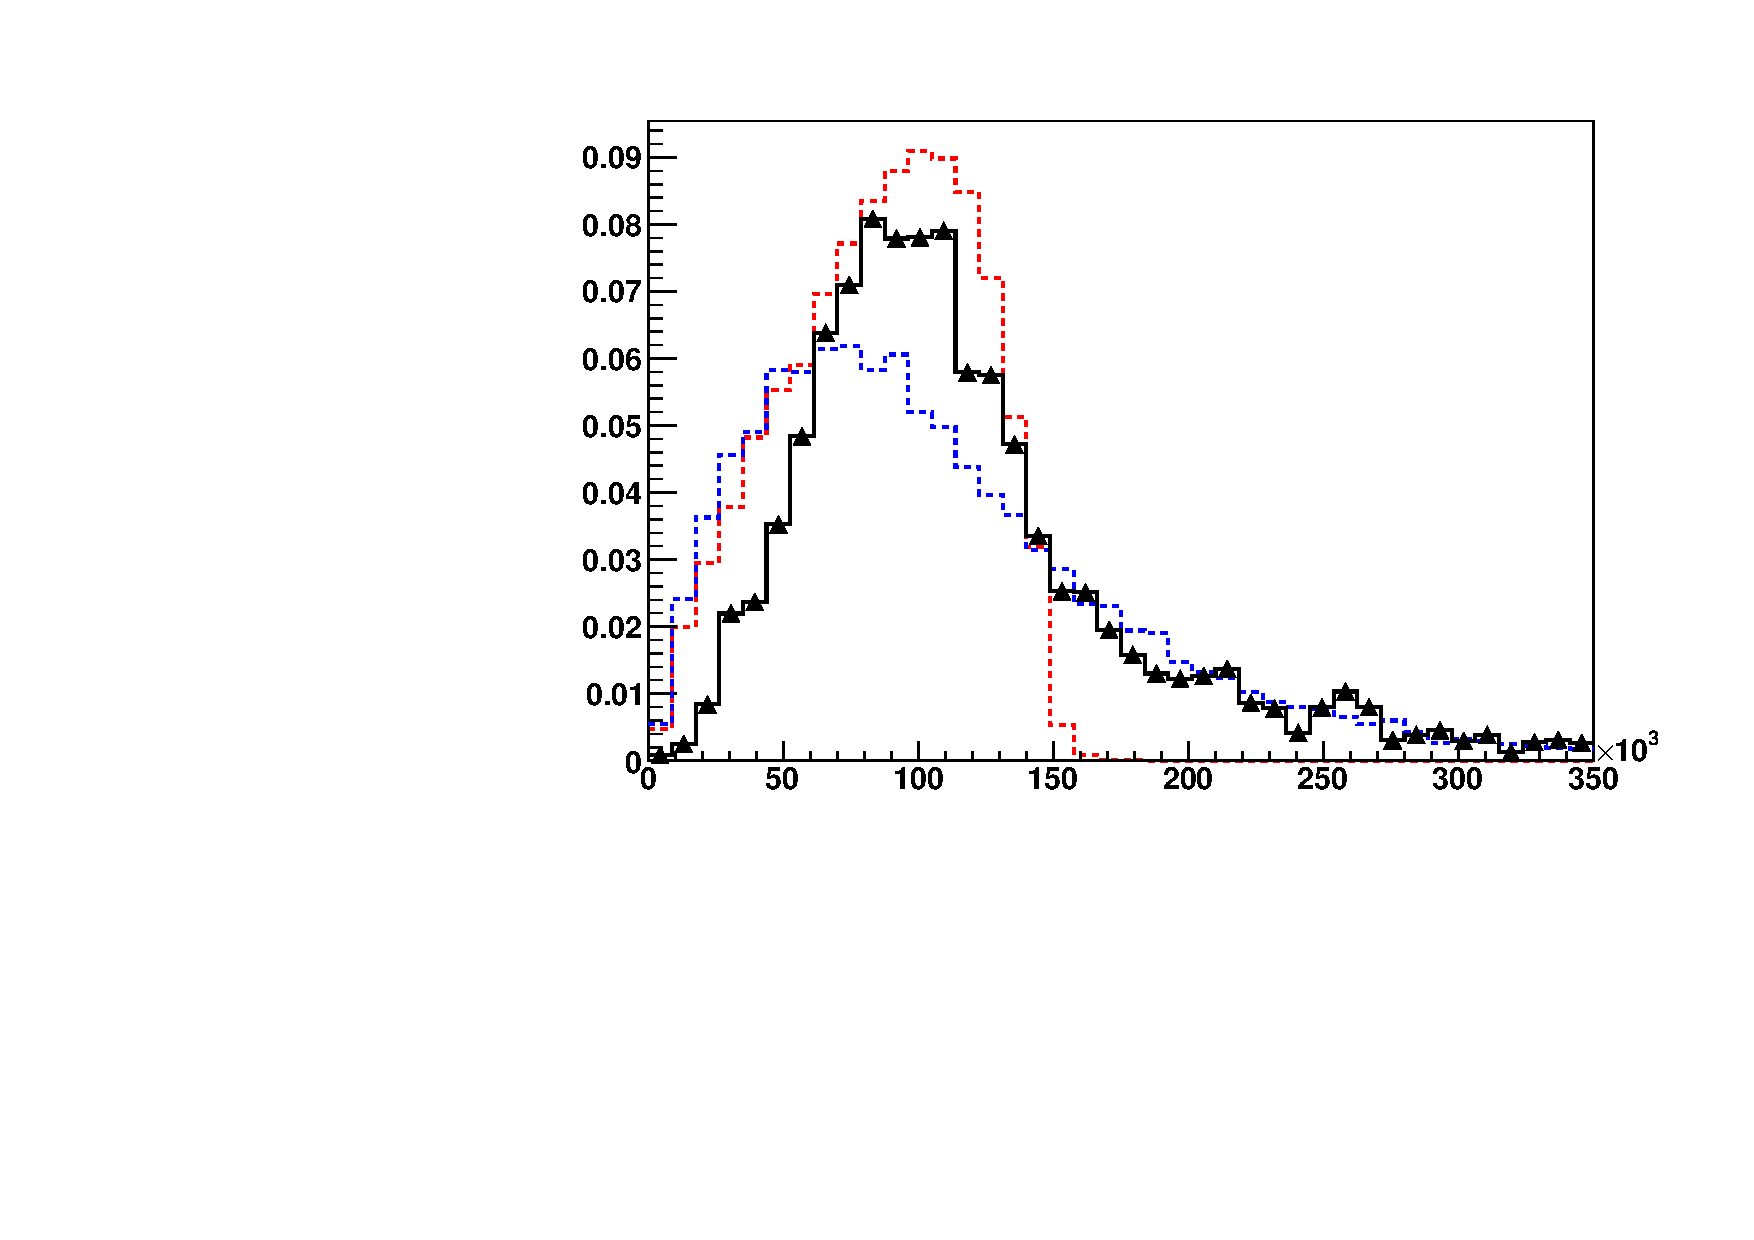
\includegraphics[width=100mm]{f/InvariantMassLepBjet}
     \end{center}
     \caption{Invariant mass distribution for lepton-jet pairings. The correct pairing is shown in red, the incorrect pairing is shown in blue. The data is shown in black.}
     \label{fig:lep_jet_mass}
    \end{figure}
%InvariantMassLepBjet


Due to the loss of statistics in KLFitter and Topology by only considering two jets, neutrino weighting still reconstructs an absolute number of events similar to that of KLFitter and Topology and no clear advantage exists between the methods. In principle all three could include the positive aspects of the others, resulting in one inclusive algorithms with higher performance than any algorithm alone. To date no such algorithm exists.


\subsubsection{Application of b-tagging}
\label{sec:btagged_selection}
The requirement of one or more b-tagged jets in an event does much to aid in background rejection but at the cost of statistics ($\sim35\%$ for two b-tags). In events at the LHC it is common for there to be higher jet multiplicities than would arise from the LO hard scatter alone. This may be due to initial and final state gluon radiation (in the case of higher order corrections) or poorly suppressed pile up. In \ttbar\ events, one might expect that the addition of b-tagging would aid in final state reconstruction, by identifying the jets from the top decay and rejecting other contributions. The reconstruction efficiency would be expected to increase for the same reason, with less jets to confuse the reconstruction it should perform better. In reality this is not the case as can be seen in table \ref{tab:nu_comparison}. The fraction of solved events that matched the truth \ttbar\ four momenta within a $\Delta R$ cone of 0.4 does not increase with the addition of b-tags. The reason for this counter intuitive result can be understood with an example.

\begin{figure}[htbp!]
     \begin{center}
     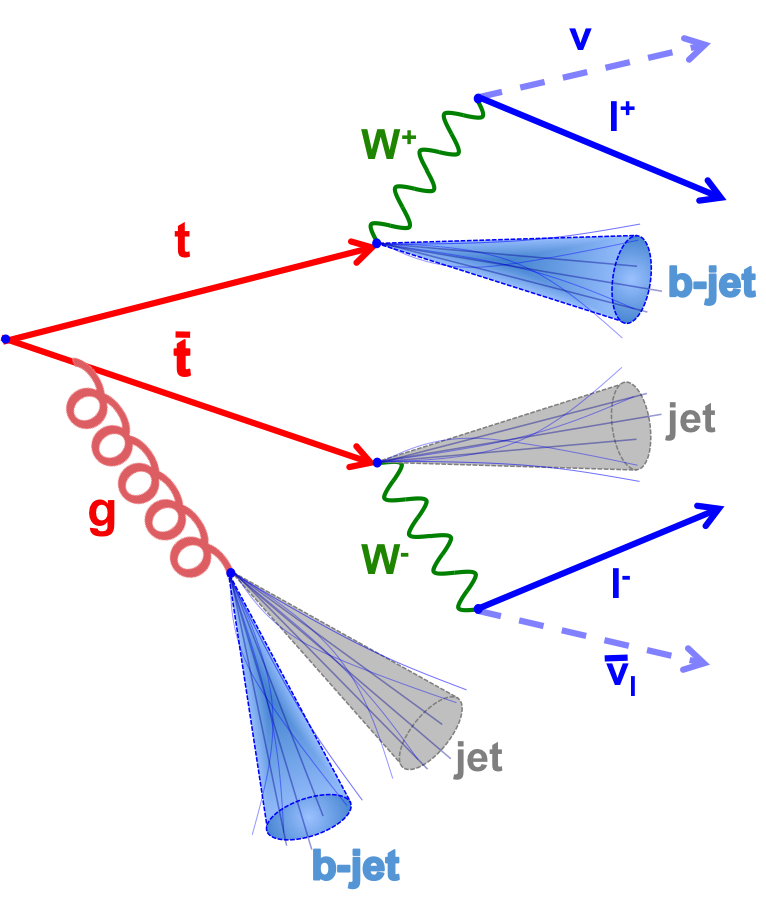
\includegraphics[width=75mm]{f/top_gluon_emission}
     \end{center}
     \caption{Cartoon showing a dileptonic \ttbar\ event where an additional jet from gluon final state radiation has been incorrectly identified as one of the b-jets coming from the top decay.}
     \label{fig:dilepton_cartoon}
    \end{figure}

\begin{figure}[htbp!]
     \begin{center}
     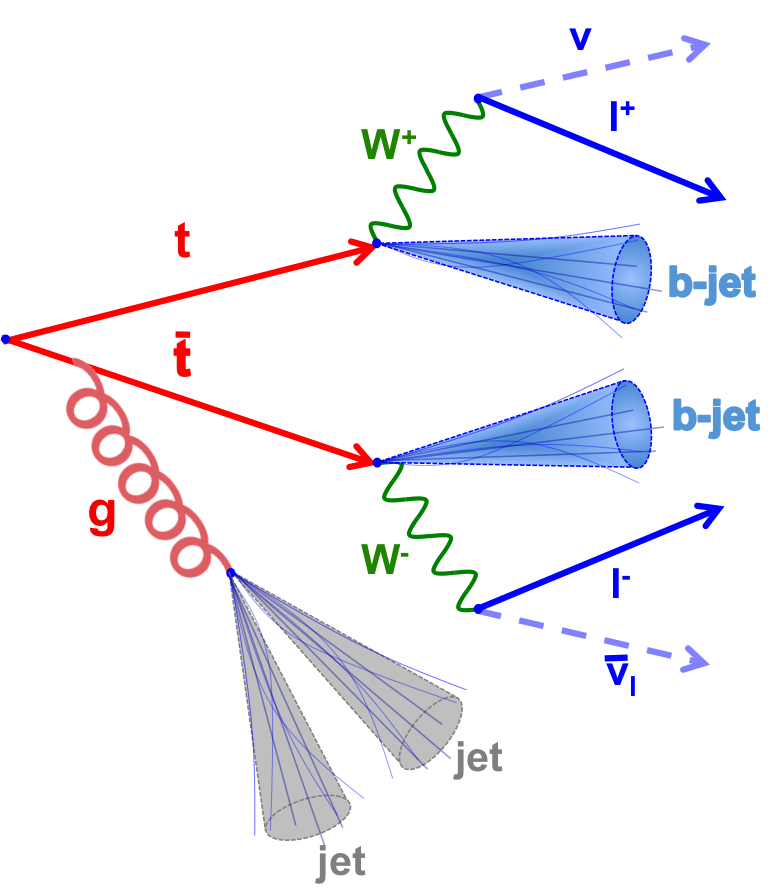
\includegraphics[width=75mm]{f/top_gluon_emission_2}
     \end{center}
     \caption{Cartoon showing a dileptonic \ttbar\ event where both b-jets were identified as coming from the top decay.}
     \label{fig:dilepton_cartoon2}
    \end{figure}

Let us imagine that we have a dileptonic \ttbar\ event in our signal MC, with at least one additional jet (3+ total). Two jets are tagged as having b-flavour and a cartoon of this event can be seen in figure \ref{fig:dilepton_cartoon}. We naturally select the two b-tagged jets and only use these in the neutrino weighting algorithm, the non b-tagged jets are not considered. The reconstruction performs poorly, and when we examine the true \ttbar\ 4-vectors we find that we have not reconstructed the system correctly. Why did this happen? One of the b-tagged jets did not come from the hard scatter, and as a result of only allowing the neutrino weighting algorithm to consider these jets it could not find the correct solution; each solution it did provide (if any) had low weights. Now let us imagine that we considered all possible combinations of jets. The two b-tagged jets still give us solutions with low weight, but now when we consider the non b-tagged jet and look at all possible combinations of jets we obtain solutions with very high weight, peaking around the true values of neutrino psuedo rapidity such as in figure \ref{top_nuweights}. Clearly we have now included the correct jet pair. When we take the average solution of all jet pairings we guarantee that we will at least examine the correct pairing, and will not be restrained by effects such as miss-tagging.

We must also consider the situation where both b-tagged jets did come from the \ttbar\ and the additional jets are not considered in the reconstruction. In this case we have removed the chance of these incorrect jets contributing fake solutions with high weights, and therefore our reconstruction efficiency would increase.

In reality both situations occur and interfere with each other, resulting in no overall improvement in the reconstruction efficiency with the addiiton of b-tagging, demonstrated in table \ref{tab:nueff}.

By drawing this conclusion we have made several assumptions:

\begin{enumerate}
\item The weights provided by a correct jet pairing are much higher than the weights from an incorrect pairing, and by taking an average we do not suffer from dilutions due to considering many small weighted events. This is illustrated in figure \ref{fig:top_nuweights}.
\item There are a significant proportion of signal events where the two highest \pt\ b-tagged jets do not correspond to the jets arising from the b-quarks. This is shown in table \ref{tab:btag_eff}.
\end{enumerate}

\begin{table}[!h]
	\begin{center}
	\begin{tabular}{ c c c c }
	\hline
	Matching Efficiency & $p_T$ ordered & B-Tag ($p_T$ ordered) & B-Tag (weight ordered) \\
	\hline
	\ee\ channel        & 51.17 \%      & 62.12 \%              & 64.75 \%               \\
	\mumu\ channel      & 52.36 \%      & 63.10 \%              & 65.70 \%               \\
	\emu\ channel       & 54.68 \%      & 64.79 \%              & 67.20 \%               \\
	\hline
	\end{tabular}
	\end{center}
	\caption{Table of reconstructed level particles matched to truth particles. Leptons are required to be matched to a truth lepton within a $\Delta R$ cone of 0.1 and jets are required to be matched to one of the truth b-jets within a $\Delta R$ cone of $0.3$. $p_T$ ordered efficiency is defined as the number of times the two highest $p_T$ jets match the truth b-quarks. B-Tag ($p_T$ ordered) is defined as the number of times the two highest $p_T$ b-tagged jets match the truth b-quarks. B-Tag (weight ordered) is defined as the number of events where two jets with the highest weighted b-tagged jets match the truth b-quarks. In all cases, when only one b-tagged jet exists, the second jet is taken to be the highest $p_T$ non b-tagged jet. }
	\label{tab:btag_eff}
\end{table}

We performed many tests on neutrino weighting with and without b-tagging, summarised in table \ref{tab:nueff}. The relative efficiency of neutrino weighting remains constant, regardless of how many b-tags are applied. We can therefore conclude that overall the addition of b-tagging serves only to suppress background in the selection, and has little effect on the net result of neutrino weighting other than to reduce the number of true signal events that we consider (though event-by-event results can be quite different). The inclusion of extra jets is not detrimental to neutrino weighting as these jets tend to produce results with low weights. This is a unique feature amongst all other \ttbar\ reconstruction algorithms that have been studied. It allows neutrino weighting to consider the full dilepton sample inclusive of all jets; a feature that is simply not available in other methods. 

\subsubsection{Why does neutrino weighting fail?}
The efficiencies described in table \ref{tab:nueff} may seem low, however it is important to understand the difference between inefficiencies caused by limitations of the algorithm and inefficiencies caused by limitations in the event selection. One important factor is that not all hard partons are inside the detector acceptance after reconstruction, but the event may still pass the event selection. If a b-quark is produced at high $\eta$ it is not detected but the event is still likely to pass the selections if there are additional pile-up jets that have not been suppressed. In these cases, we never have the opportunity to correctly use the correct jets in the reconstruction. 

Gluon emission in the final state also produces a situation where we cannot correctly solve the system, our reconstructed four vector for the top quark will have missing momentum and will not match the truth top. 

Finally, our assumption of the range of possible neutrino $\eta$ may not have sufficiently broad and the true neutrino $|\eta|$ may have been greater than 4.0. In MC studies this was shown to occur in less than 0.0001\% of unmatched or failed reconstructions.

All of these features will result in an inefficiency that was not due to shortcomings in the reconstruction algorithm. Some of these effects can be corrected for in the MC with the application of cuts, achieving efficiencies as high as $\sim45\%$ but these require MC truth information and could not be applied on data.

%\subsubsection*{Kinematic Solution}
%\begin{equation*}
 % \begin{aligned}
  %  \\
   % p^{i} & = (E^{i}, \vec{\textbf{p}}^{i}) = (E^{i}, p_{x}^{i}, p_{y}^{i}, p_{z}^{i}) \\
    %p^{i} & = \mbox{contravariant 4-vector of particle of type i}\\
    %m_{i} & = \mbox{mass of particle of type i}\\
    %h = c & = 1 \text{          (working in natual units)} \\
    %\\
    %p_t^i &  = \sqrt{p^{i2}_x + p^{i2}_y} \\
    %\\
  %\end{aligned}
%\end{equation*}
%We may begin with a series of Kinematic constraints:
%\begin{equation}
 % \begin{aligned}
   % \\
   % m_{W} & =(p^{l} + p^{\nu})^2 \\
   % m_{t} & =(p^{l} + p^{\nu} + p^{b})^2 \\
    %\\
  %\end{aligned}
  %\label{nuW:mass_constraint}
%\end{equation}
%We also know from experiment the following quantities:
%\begin{equation*}
 % \begin{aligned}
  %  \\
   % m_{b} = m_{\bar{b}} & = 4.5\GeV \\
   % m_{W} & = 80.4\GeV \\
   %% m_{t} & = 172.5\GeV \\
   % m_{l^+} = m_{l^-} & \approx 0.0\GeV \\
   % m_{\nu} = m_{\bar{\nu}} & \approx 0.0\GeV \\
    %p^{b}, p^{\bar{b}}, p^{l+}, p^{l-} & \mbox{ measured per event}\\
   % \\
    %\end{aligned}
%\end{equation*}
%Although we measure the transverse components of the two neutrino energies via missing energy in the event, this is not used in the kinematic reconstruction but is used as a figure of merit later in the reconstruction procedure. From equation \ref{nuW:mass_constraint} we can expand the equations for $m_{W}$:
%\begin{equation}
  %\begin{aligned}
 %   \\
  %  m_{W}^2 = (E^l + E^{\nu})^2 - (\vec{\textbf{p}}^{l} + \vec{\textbf{p}}^{\nu})^2 & = E^{l^2} + E^{\nu^2} - \vec{\textbf{p}}^{l^2} - \vec{\textbf{p}}^{\nu^2} + 2E^l E^{\nu} - 2\vec{\textbf{p}}^{l} \vec{\textbf{p}}^{\nu} \\
   %  & = 2(E^l E^{\nu} - \vec{\textbf{p}}^{l} \vec{\textbf{p}}^{\nu})\\
    %\\
   % \end{aligned}
%\end{equation}
%We may rearrange this equation for $E^{\nu}$:
%\begin{equation}
 % \\
  %E^{\nu} = |\vec{\textbf{p}}^{\nu}| = \frac{1}{E^l}(\frac{m_{W}^2}{2} + \vec{\textbf{p}}^{l} \vec{\textbf{p}}^{\nu})\\
  %\\
  %\label{nuW:nu_energy_1}%
%\end{equation}
%Similarly we can derive an equivalent equation from the top mass constraint in equation \ref{nuW:mass_constraint}:
%\begin{equation}
 % \begin{aligned}
   % \\
   % m_{t}^2 & = (E^l + E^{\nu} + E^b)^2 - (\vec{\textbf{p}}^{l} + \vec{\textbf{p}}^{\nu} + \vec{\textbf{p}}^{b})^2 \\
    %        & = m_{W}^2 + m_{b}^2 + 2(E^l E^b + E^{\nu} E^{b} - \vec{\textbf{p}}^{l} \vec{\textbf{p}}^{b} - \vec{\textbf{p}}^{\nu} \vec{\textbf{p}}^{b}) \\
    %E^{\nu} & = |\vec{\textbf{p}}^{\nu}| = \frac{m_{t}^2 - m_{W}^2 - m_{b}^2 - 2 p^l p^b}{2 E^b} + \frac{\vec{\textbf{p}}^{\nu} \vec{\textbf{p}}^{b}}{E^b} \\
    %\\
  %\end{aligned}
  %\label{nuW:nu_energy_2}
%\end{equation}
%It is useful to boost into the frame of reference where the neutrinos have no momentum in the direction of the beam, i.e. $p^{\nu}_z = 0$\GeV:
%\begin{equation}
%\begin{aligned}
%\\
%L = 
%\begin{pmatrix}
%\cosh{\eta^{\nu}} & 0 & 0 & -\sinh{\eta^{\nu}} \\
 %       0         & 1 & 0 & 0 \\%
%	0         & 0 & 1 & 0 \\
%-\sinh{\eta^{\nu}}& 0 & 0 & \cosh{\eta^{\nu}}\\
%\end{pmatrix}
%\\
%\end{aligned}
%\end{equation}
%Applying this boost to equation \ref{nuW:nu_energy_1} gives:
%\begin{equation}
%\begin{aligned}
%\\
 % p^{\nu}_T = \frac{m_{W}^2}{2 E^{l^{\prime}}} + \frac{p^l_x p^{\nu}_x}{E^{l^{\prime}}} + \frac{p^l_y p^{\nu}_y}{E^{l^{\prime}}}\\
%\\
%\end{aligned}
%\label{nuW:pt_1}
%^\end{equation}
%where
%\begin{equation}
%\begin{aligned}
%E^{l^{\prime}} = E^l\cosh\eta^{\nu} - p^l_x\sinh{\eta^{\nu}}\\
%\\
%\end{aligned}
%\end{equation}
%Similarly applying this boost to equation \ref{nuW:nu_energy_2} yields:
%\begin{equation}
%\begin{aligned}
%\\
%p^{\nu}_T = \frac{m_{t}^2 - m_W^2 - m_b^2 - 2 p^l p^b}{2 E^{b^{\prime}}} + \frac{p^{\nu}_x p^b_x +  p^{\nu}_y p^b_y}{E^{b^{\prime}}}\\
%\\
%\end{aligned}
%\label{nuW:pt_2}
%\end{equation}
%where
%\begin{equation}
%\begin{aligned}
%E^{b^{\prime}} = E^b\cosh\eta^{\nu} - p^b_x\sinh{\eta^{\nu}}\\
%\\
%\end{aligned}
%\end{equation}
%Equations \ref{nuW:pt_1} and \ref{nuW:pt_2} are equivalent and after solving for $p^{\nu}_x$ one obtains the linear equation:
%\begin{equation}
%\begin{aligned}
%\\
%p^{\nu}_x = ap^{\nu}_y + b \\
%\\
%\end{aligned}
%\label{nuW:px}
%\end{equation}
%where:
%\begin{equation}
%\begin{aligned}
%\\
%a  & = \frac{p^l_y E^{b^{\prime}} - p^b_y E^{l^{\prime}}}{p^b_x E^{l^{\prime}} - p^l_x E^{b^{\prime}}} \\
%\\
%b  & = \frac{E^{l^{\prime}}(m_t^2 - m_W^2 -m_b^2 - 2p^lb^l) - E^{b^{\prime}}m_W^2}{2(p^l_x E^{b^{\prime}} - p^b_x E^{l^{\prime}})}\\
%\\
%\end{aligned}
%\end{equation}
%If we use equation \ref{nuW:px} and the definition of $p_T$ we can rearrange equation \ref{nuW:pt_1} to get:
%\begin{equation}
%\begin{aligned}
%\\
%\sqrt{(a^2 + 1)p^{\nu}_y + 2abp^{\nu}_y + b^2} = \frac{m_W^2}{2E^{l^{\prime}}} + \frac{p^l_x}{E^{l^{\prime}}}(ap^{\nu}_y + b) + \frac{p^l_y}{E^{l^{\prime}}}p^{\nu}_y \\
%\\
%\end{aligned}
%\label{nuW:quad}
%\end{equation}
%If we square equation \ref{nuW:quad} we can obtain a quadratic equation in terms of $p^{\nu}_y$ in the form:
%\begin{equation}
%\begin{aligned}
%\\
%cp^{\nu2}_y + dp^{\nu}_y + f = 0\\
%\\
%\end{aligned}
%\label{nuW:quad2}
%\end{equation}
%with
%\begin{equation}
%\begin{aligned}
%\\
%c & = a^2 + 1 - (\frac{p^l_x}{E^{l^{\prime}}}a + \frac{p^l_y}{E^{l^{\prime}}})^2 \\
%\\
%d & = 2ab - 2(\frac{m_W^2}{2E^{l^{\prime}}} + \frac{p^l_x}{E^{l^{\prime}}}b)(\frac{p^l_x}{E^{l^{\prime}}}a + \frac{p^l_y}{E^{l^{\prime}}})\\
%\\
%f & = b^2 - (\frac{m_W^2}{2E^{l^{\prime}}} + \frac{p^l_x}{E^{l^{\prime}}}b)^2\\
%\\
%\end{aligned}
%\end{equation}
%Equation \ref{nuW:quad2} has two roots. Since we only consider real roots to be physical equation \ref{nuW:quad2} has either 0, 1 or 2 real solutions for $p^{\nu}_y$.
%\begin{equation}
%\begin{aligned}
%\\
%p^{\nu}_y = -\frac{d}{2c}\pm\frac{1}{2c}\sqrt{d^2 - 4cf}\\
%\\
%\end{aligned}
%\end{equation}
%
%Original derivtion taken from (Reference D0 Thesis).
%
